% Options for packages loaded elsewhere
\PassOptionsToPackage{unicode}{hyperref}
\PassOptionsToPackage{hyphens}{url}
%
\documentclass[
]{book}
\usepackage{lmodern}
\usepackage{amssymb,amsmath}
\usepackage{ifxetex,ifluatex}
\ifnum 0\ifxetex 1\fi\ifluatex 1\fi=0 % if pdftex
  \usepackage[T1]{fontenc}
  \usepackage[utf8]{inputenc}
  \usepackage{textcomp} % provide euro and other symbols
\else % if luatex or xetex
  \usepackage{unicode-math}
  \defaultfontfeatures{Scale=MatchLowercase}
  \defaultfontfeatures[\rmfamily]{Ligatures=TeX,Scale=1}
\fi
% Use upquote if available, for straight quotes in verbatim environments
\IfFileExists{upquote.sty}{\usepackage{upquote}}{}
\IfFileExists{microtype.sty}{% use microtype if available
  \usepackage[]{microtype}
  \UseMicrotypeSet[protrusion]{basicmath} % disable protrusion for tt fonts
}{}
\makeatletter
\@ifundefined{KOMAClassName}{% if non-KOMA class
  \IfFileExists{parskip.sty}{%
    \usepackage{parskip}
  }{% else
    \setlength{\parindent}{0pt}
    \setlength{\parskip}{6pt plus 2pt minus 1pt}}
}{% if KOMA class
  \KOMAoptions{parskip=half}}
\makeatother
\usepackage{xcolor}
\IfFileExists{xurl.sty}{\usepackage{xurl}}{} % add URL line breaks if available
\IfFileExists{bookmark.sty}{\usepackage{bookmark}}{\usepackage{hyperref}}
\hypersetup{
  pdftitle={ShinyDataSHIELD User's Guide},
  pdfauthor={Escribà Montagut, Xavier; González, Juan R.},
  hidelinks,
  pdfcreator={LaTeX via pandoc}}
\urlstyle{same} % disable monospaced font for URLs
\usepackage{color}
\usepackage{fancyvrb}
\newcommand{\VerbBar}{|}
\newcommand{\VERB}{\Verb[commandchars=\\\{\}]}
\DefineVerbatimEnvironment{Highlighting}{Verbatim}{commandchars=\\\{\}}
% Add ',fontsize=\small' for more characters per line
\usepackage{framed}
\definecolor{shadecolor}{RGB}{248,248,248}
\newenvironment{Shaded}{\begin{snugshade}}{\end{snugshade}}
\newcommand{\AlertTok}[1]{\textcolor[rgb]{0.94,0.16,0.16}{#1}}
\newcommand{\AnnotationTok}[1]{\textcolor[rgb]{0.56,0.35,0.01}{\textbf{\textit{#1}}}}
\newcommand{\AttributeTok}[1]{\textcolor[rgb]{0.77,0.63,0.00}{#1}}
\newcommand{\BaseNTok}[1]{\textcolor[rgb]{0.00,0.00,0.81}{#1}}
\newcommand{\BuiltInTok}[1]{#1}
\newcommand{\CharTok}[1]{\textcolor[rgb]{0.31,0.60,0.02}{#1}}
\newcommand{\CommentTok}[1]{\textcolor[rgb]{0.56,0.35,0.01}{\textit{#1}}}
\newcommand{\CommentVarTok}[1]{\textcolor[rgb]{0.56,0.35,0.01}{\textbf{\textit{#1}}}}
\newcommand{\ConstantTok}[1]{\textcolor[rgb]{0.00,0.00,0.00}{#1}}
\newcommand{\ControlFlowTok}[1]{\textcolor[rgb]{0.13,0.29,0.53}{\textbf{#1}}}
\newcommand{\DataTypeTok}[1]{\textcolor[rgb]{0.13,0.29,0.53}{#1}}
\newcommand{\DecValTok}[1]{\textcolor[rgb]{0.00,0.00,0.81}{#1}}
\newcommand{\DocumentationTok}[1]{\textcolor[rgb]{0.56,0.35,0.01}{\textbf{\textit{#1}}}}
\newcommand{\ErrorTok}[1]{\textcolor[rgb]{0.64,0.00,0.00}{\textbf{#1}}}
\newcommand{\ExtensionTok}[1]{#1}
\newcommand{\FloatTok}[1]{\textcolor[rgb]{0.00,0.00,0.81}{#1}}
\newcommand{\FunctionTok}[1]{\textcolor[rgb]{0.00,0.00,0.00}{#1}}
\newcommand{\ImportTok}[1]{#1}
\newcommand{\InformationTok}[1]{\textcolor[rgb]{0.56,0.35,0.01}{\textbf{\textit{#1}}}}
\newcommand{\KeywordTok}[1]{\textcolor[rgb]{0.13,0.29,0.53}{\textbf{#1}}}
\newcommand{\NormalTok}[1]{#1}
\newcommand{\OperatorTok}[1]{\textcolor[rgb]{0.81,0.36,0.00}{\textbf{#1}}}
\newcommand{\OtherTok}[1]{\textcolor[rgb]{0.56,0.35,0.01}{#1}}
\newcommand{\PreprocessorTok}[1]{\textcolor[rgb]{0.56,0.35,0.01}{\textit{#1}}}
\newcommand{\RegionMarkerTok}[1]{#1}
\newcommand{\SpecialCharTok}[1]{\textcolor[rgb]{0.00,0.00,0.00}{#1}}
\newcommand{\SpecialStringTok}[1]{\textcolor[rgb]{0.31,0.60,0.02}{#1}}
\newcommand{\StringTok}[1]{\textcolor[rgb]{0.31,0.60,0.02}{#1}}
\newcommand{\VariableTok}[1]{\textcolor[rgb]{0.00,0.00,0.00}{#1}}
\newcommand{\VerbatimStringTok}[1]{\textcolor[rgb]{0.31,0.60,0.02}{#1}}
\newcommand{\WarningTok}[1]{\textcolor[rgb]{0.56,0.35,0.01}{\textbf{\textit{#1}}}}
\usepackage{longtable,booktabs}
% Correct order of tables after \paragraph or \subparagraph
\usepackage{etoolbox}
\makeatletter
\patchcmd\longtable{\par}{\if@noskipsec\mbox{}\fi\par}{}{}
\makeatother
% Allow footnotes in longtable head/foot
\IfFileExists{footnotehyper.sty}{\usepackage{footnotehyper}}{\usepackage{footnote}}
\makesavenoteenv{longtable}
\usepackage{graphicx,grffile}
\makeatletter
\def\maxwidth{\ifdim\Gin@nat@width>\linewidth\linewidth\else\Gin@nat@width\fi}
\def\maxheight{\ifdim\Gin@nat@height>\textheight\textheight\else\Gin@nat@height\fi}
\makeatother
% Scale images if necessary, so that they will not overflow the page
% margins by default, and it is still possible to overwrite the defaults
% using explicit options in \includegraphics[width, height, ...]{}
\setkeys{Gin}{width=\maxwidth,height=\maxheight,keepaspectratio}
% Set default figure placement to htbp
\makeatletter
\def\fps@figure{htbp}
\makeatother
\setlength{\emergencystretch}{3em} % prevent overfull lines
\providecommand{\tightlist}{%
  \setlength{\itemsep}{0pt}\setlength{\parskip}{0pt}}
\setcounter{secnumdepth}{5}
\usepackage{booktabs}
\usepackage[]{natbib}
\bibliographystyle{apalike}

\title{ShinyDataSHIELD User's Guide}
\author{Escribà Montagut, Xavier; González, Juan R.}
\date{2020-09-30}

\begin{document}
\maketitle

{
\setcounter{tocdepth}{1}
\tableofcontents
}
\hypertarget{overview}{%
\chapter{Overview}\label{overview}}


\includegraphics[width=0.5\textwidth,height=\textheight]{images/ds_logo.png}

ShinyDataSHIELD is a non-disclosive data analysis toolbox powered by DataSHIELD with the following features:

\begin{itemize}
\tightlist
\item
  Descriptive statistics: Summary, scatter plots, histograms and heatmaps of table variables.
\item
  Statistic models: GLM and GLMer model fittings
\item
  Omic analysis: GWAS, LIMMA, \ldots{} using different types of resources (VCF files, PLINK, RSE, eSets)
\end{itemize}

The features available on ShinyDataSHIELD are powered by different packages of the DataSHIELD project (dsBaseClient and dsOmicsClient), it uses them in a seamless way so the final user of ShinyDataSHIELD can perform all the included studies without writing a single line of code and get all the resulting figures and tables by the click of a button.

\hypertarget{setup}{%
\chapter{Setup}\label{setup}}

In order to use ShinyDataSHIELD, Docker is required. On a Linux / Mac OS X machine it can be installed without any complications as any other application, on Windows systems however it can be a little bit more troubling, there are many online resources to help. Please refer to the following links to help the installation of Docker on a Windows system \href{https://docs.docker.com/docker-for-windows/install-windows-home/}{1}, \href{https://blog.nillsf.com/index.php/2020/02/17/setting-up-wsl2-windows-terminal-and-oh-my-zsh/}{2}, \href{https://docs.docker.com/docker-for-windows/wsl/}{3}.

To download and launch ShinyDataSHIELD, execute the following command on a bash terminal(make sure Docker is running, if not search for the \texttt{Docker\ Desktop} app and launch it).

\begin{Shaded}
\begin{Highlighting}[]
\ExtensionTok{docker}\NormalTok{ run --rm -p 80:80 brgelab/shiny-data-shield}
\end{Highlighting}
\end{Shaded}

This command will download the Docker image of ShinyDataSHIELD (be aware it weights \textasciitilde{} 1.5 GB, so if your internet connection is slow it may take a while) and run a container with it. The container will be exposed on the local port 80 and it will render on that port the application itself, so to start using ShinyDataSHIELD open your web browser of choice and go to the site

\begin{Shaded}
\begin{Highlighting}[]
\ExtensionTok{localhost}\NormalTok{:80}
\end{Highlighting}
\end{Shaded}

At the beginning it may take some time for the application to render, this is because all the needed R libraries are being loaded, to be sure the container is actually working, take a look at the terminal where you inputed the Docker command, there you will see all the R verbose stating the libraries are being loaded.

Once the user has finished using ShinyDataSHIELD, the container needs to be stopped to avoid wasting CPU resources, to do so, input the following command on a bash terminal (the command needs to be inputed on a new bash window):

\begin{Shaded}
\begin{Highlighting}[]
\ExtensionTok{docker}\NormalTok{ container ls}
\end{Highlighting}
\end{Shaded}

This will prompt all the running containers, find the one with the NAMES \texttt{brgelab/shiny-data-shield} and copy it's CONTAINER ID, then input the following bash command:

\begin{Shaded}
\begin{Highlighting}[]
\ExtensionTok{docker}\NormalTok{ stop xxxxxxxxxxxx}
\end{Highlighting}
\end{Shaded}

Where xxxxxxxxxxxx is the CONTAINER ID.

To run the application again, just enter the first bash command (\texttt{docker\ run\ -\/-rm\ -p\ 80:80\ brgelab/shiny-data-shield}), since it has already been downloaded, the application is cached on the computer and it will launch straight away. If the user wants to remove the Docker image from the computer, input the following bash command:

\begin{Shaded}
\begin{Highlighting}[]
\ExtensionTok{docker}\NormalTok{ image rm brgelab/exposome-shiny}
\end{Highlighting}
\end{Shaded}

If the user wants to download the actual source code of the Shiny, install all the required packages and launch it locally on it's machine, feel free to download it \href{https://github.com/isglobal-brge/dsOmicsShiny}{from Github}. There's a script called \texttt{installer.R} at the root of the repository with a short installer of all the required packages. Please note that the installer script may fail depending on the R version and others, for that reason is advised to always run the Docker version of ShinyDataSHIELD, as it only requires a single terminal command and will work no matter what.

\hypertarget{r-packages}{%
\chapter{R packages}\label{r-packages}}

The packages that contain the main functionalities of ShinyDataSHIELD are the following.

\begin{itemize}
\tightlist
\item
  \href{https://github.com/datashield/DSI}{DSI}: The DataSHIELD Interface (DSI) handles the connections to the databases.
\item
  \href{https://github.com/datashield/DSOpal}{DSOpal}: DSOpal is an extension of DSI to connecto to Opal servers.
\item
  \href{https://github.com/datashield/dsBaseClient}{dsBaseClient}: Implementation of the base package R functions to obtain non-disclosive returns from the Opal servers (Example: Base package function \texttt{as.factor} is implemented as \texttt{ds.asFactor}).
\item
  \href{https://github.com/isglobal-brge/dsOmicsClient}{dsOmicsClient}: Functions to perform non-disclosive omic analysis using BioConductor packages on the Opal servers.
\end{itemize}

On the following table, all the packages required by ShinyDataSHIELD are shown along the versions used during development.

\begin{longtable}[]{@{}ll@{}}
\toprule
Package & Version\tabularnewline
\midrule
\endhead
DSI & 1.1.0\tabularnewline
DSOpal & 1.1.0\tabularnewline
dsBaseClient & 6.0.1\tabularnewline
dsOmicsClient & 1.0.0\tabularnewline
shinydashboard & 0.7.1\tabularnewline
shiny & 1.4.0.2\tabularnewline
shinyalert & 1.1\tabularnewline
DT & 0.13\tabularnewline
data.table & 1.12.8\tabularnewline
shinyjs & 1.1\tabularnewline
shinyBS & 0.61\tabularnewline
shinycssloaders & 0.3\tabularnewline
stringr & 1.4.0\tabularnewline
\bottomrule
\end{longtable}

\hypertarget{functionalities}{%
\chapter{Functionalities}\label{functionalities}}

Along this section, an overview of the functionalities implemented on ShinyDataSHIELD is given. There's information about how to use the funcionalities as well as some limitations or constraints to take into account when using ShinyDataSHIELD.

\hypertarget{data-entry}{%
\section{Data entry}\label{data-entry}}

\begin{longtable}[]{@{}l@{}}
\toprule
\begin{minipage}[b]{0.97\columnwidth}\raggedright
⚠️ DISCLAIMER\strut
\end{minipage}\tabularnewline
\midrule
\endhead
\begin{minipage}[t]{0.97\columnwidth}\raggedright
Along this section the terms \textbf{table} and \textbf{resource} are widely used, it is important noting that when the autor talks about a table, it refers to what is shown as a table on the Opal server. A resource that holds a table is called (and treated) as a resource.\strut
\end{minipage}\tabularnewline
\bottomrule
\end{longtable}

The first step to any analysis is to load the required tables or resources to the study server(s). To do so, the user has to provide the server URL and the login credentials. This will allow the application to connect to the OPAL server and retrieve all the projects and resources / tables from them. Afterwards, the user can select the desired resources / tables and load them to the study servers.

There are some limitations to how the data entry is coded in ShinyDataSHIELD:

\begin{itemize}
\tightlist
\item
  When loading multiple tables / resources on a study server, it is assumed only tables are selected or only resources, not combined.
\item
  When dealing with tables, there can only be one table per study.
\item
  A pooled study can only contain one table (or resource) per study server.
\item
  When performing a pooled study, consistency among the tables is assumed, meaning all tables share the same columns.
\item
  When loading multiple resources per study server, only one study is allowed.
\end{itemize}

The limitations can be overcome by changing the part of the code in charge of the data entry. Look at the developers guide flowcharts to get some references on which parts of the code could be altered to change the current limitations.

When loged into the Opal server, the interface shows two selectors, one is a dropdown with all the projects found on the server, the other is a dropdown (with multiple selection) with the resources / tables inside the selected project. The user has to select the project and resource(s) / table(s) that wants to load on a study server and press the ``Add study'' button.

Below the two selectors a table will be shown, on this table each line corresponds to a study server. If the user made a mistake when adding a study server, the rows on this table can be selected, and by pressing the ``Remove selected study'' button, the selected study servers will be removed.

When the desired study serveres are selected, press the ``Connect'' button to connect to them.

Following the limitations explained before, there are three different use cases.

\hypertarget{single-resource-table-approach}{%
\subsection{Single resource / table approach}\label{single-resource-table-approach}}

To perform analysis on data that is contained on a single resource / table of the server, the user has to select it from the dropdown inputs, add it to the study and connect to it.

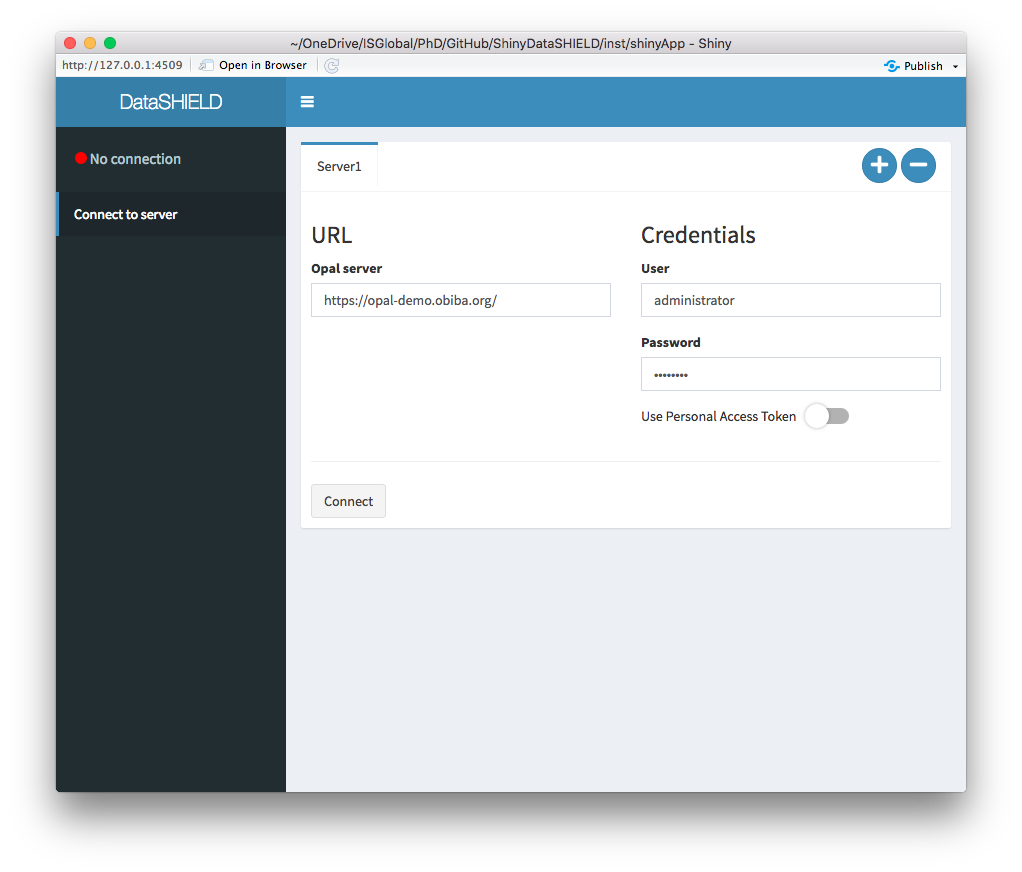
\includegraphics{images/data_entry1.png}

\hypertarget{multiple-resource-study}{%
\subsection{Multiple resource study}\label{multiple-resource-study}}

Some studies require to put more than one resource on a study server, this is the case for example of using VCF files to perform a GWAS; they require two resources, the VCF resource and the covariates resource (which is a resource that holds a plain table). For this use case, the user has to select the multiple resources from the dropdown inputs, add them to a single study and connect to it.

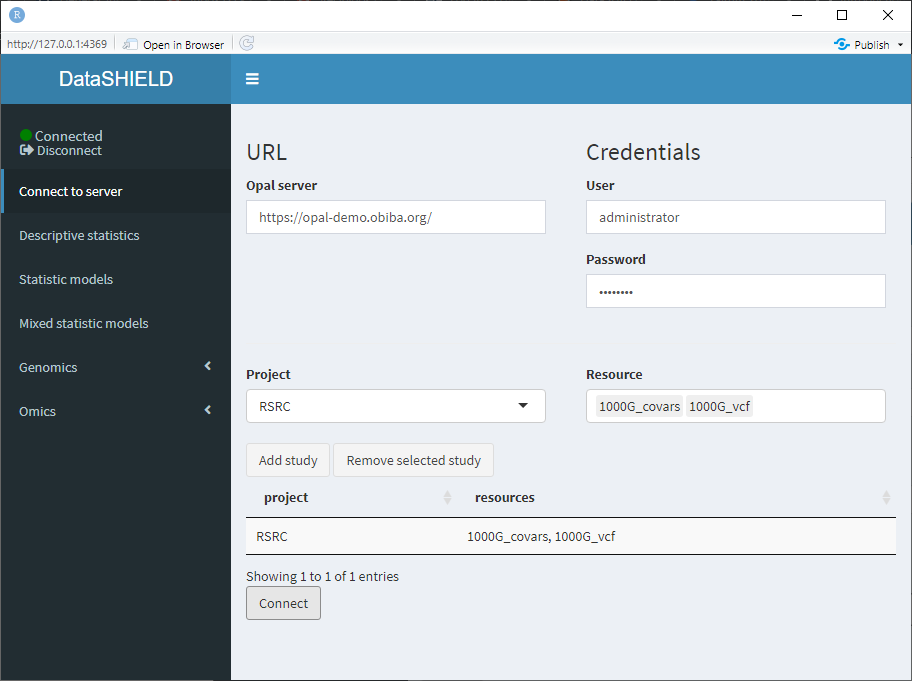
\includegraphics{images/data_entry2.png}

\hypertarget{pooled-data-approach}{%
\subsection{Pooled data approach}\label{pooled-data-approach}}

Some studies have the data distributed across multiple tables or resources that need to be pooled to perform a study. To load this kind of studies, the user has to select each different table / resource, add it to a study separately and connect to it.

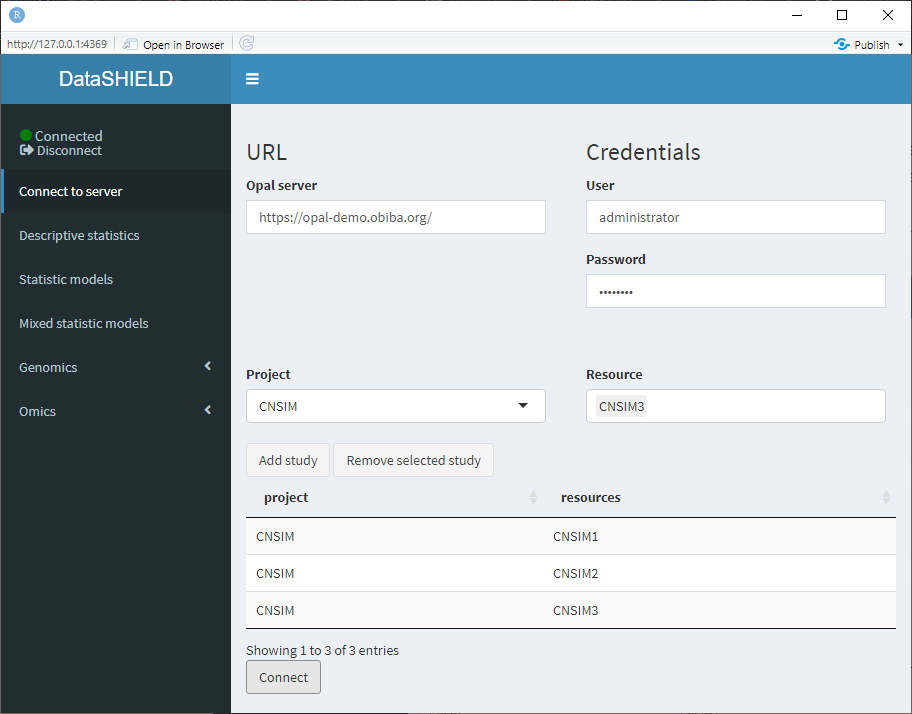
\includegraphics{images/data_entry3.png}

\hypertarget{descriptive-statistics}{%
\section{Descriptive statistics}\label{descriptive-statistics}}

The descriptive statistics functionality is available for tables as well as the following resource types:

\begin{itemize}
\tightlist
\item
  SQL tables
\item
  Tidy data files (tables): \texttt{*.csv}, \texttt{*.tsv}, etc
\item
  ExpressionSets
\item
  RangedSummarizedExperiments
\end{itemize}

When using pooled data the descriptive statistics is by default of the pooled data, however, the graphical visualizations included on descriptive statistics provide the option of showing separated plots for the different studies.

The download button will prompt a system window to select where to store the shown table, it will save it as a \texttt{*.csv}.

\hypertarget{summary}{%
\subsection{Summary}\label{summary}}

The summary provides non-disclosive insights on the different variables of the loaded data. This functionality is only available for factors and numeric variables, otherwise no table will be rendered. When the desired summary is disclosive no table will be shown (as the function call returns an Error stating that the the return is disclosive).

When the selected variable is a factor, the output shown is a count of all the different factors.

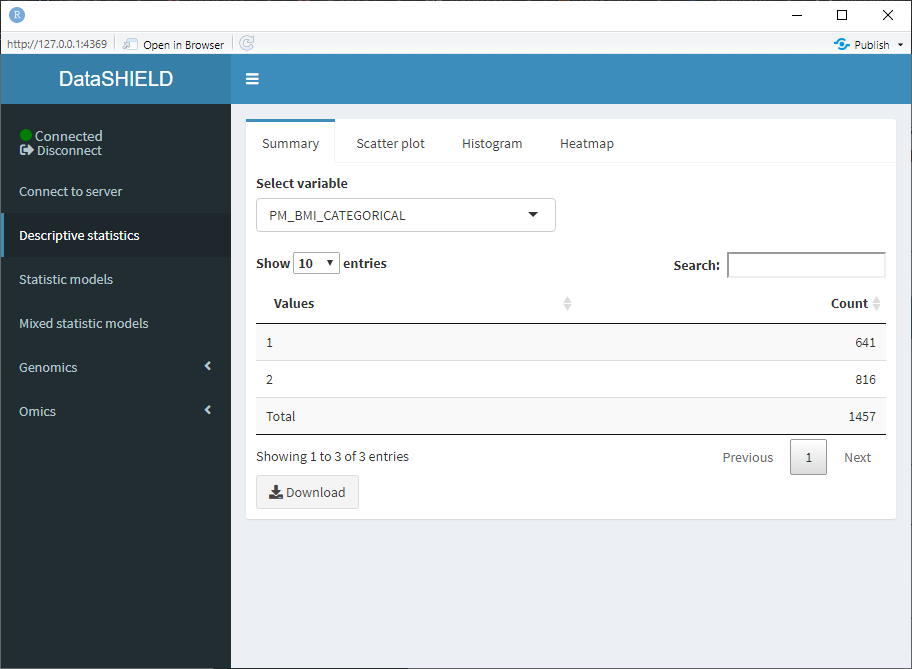
\includegraphics{images/descriptive_stats2.png}

When the selected variable is numerical, the output shown is a quantiles and mean table.

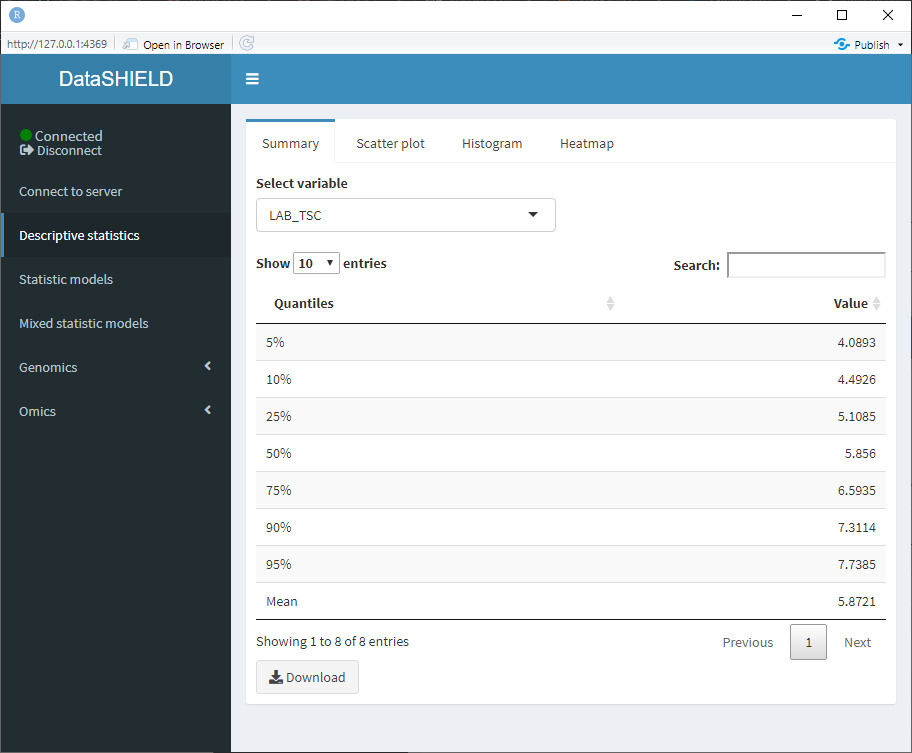
\includegraphics{images/descriptive_stats1.png}

\hypertarget{scatter-plot}{%
\subsection{Scatter plot}\label{scatter-plot}}

Create a non-disclosive scatter plot by selecting two numerical variables (one for each axis). There's the option of obtaining a pooled data plot or a different plot for each study server. The selected variables have to be numerical, otherwise the plot is not displayed and a warning message appears.

The dowload plot button saves the shown figure as a \texttt{*.png}.

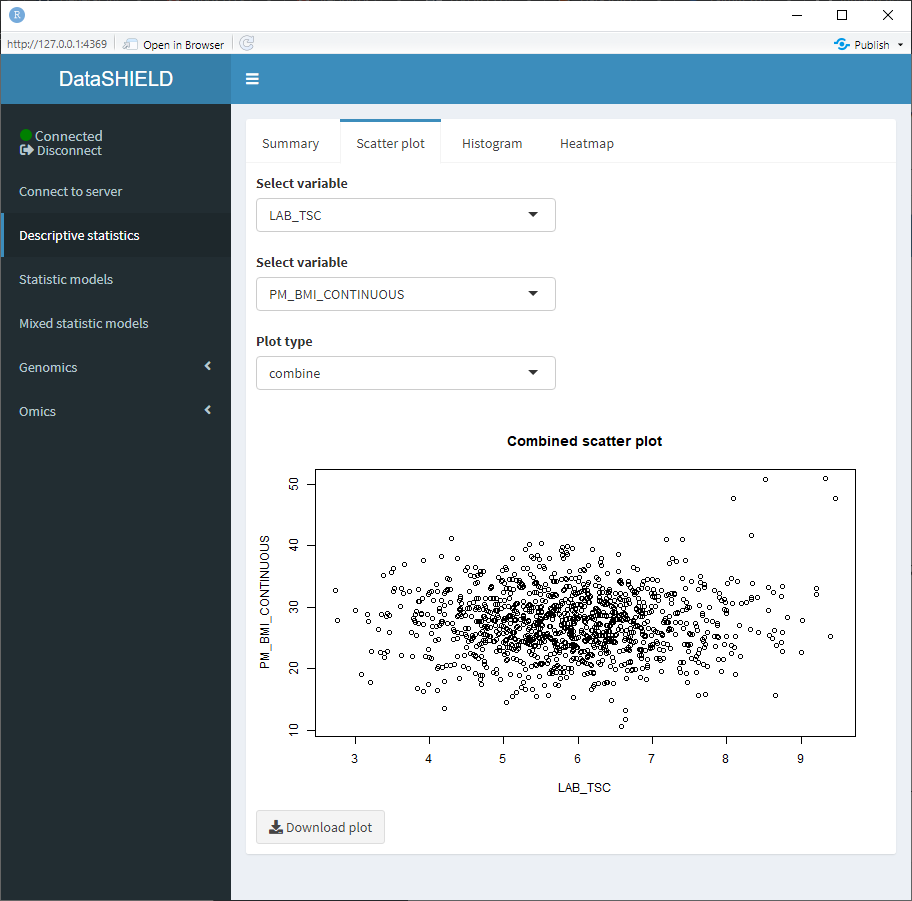
\includegraphics{images/descriptive_stats3.png}

\hypertarget{histogram}{%
\subsection{Histogram}\label{histogram}}

Create a non-disclosive histogram of a selected variable. There's the option of obtaining a pooled data plot or a different plot for each study server. The selected variable has to be numerical, otherwise the plot is not displayed and a warning message appears.

The dowload plot button saves the shown figure as a \texttt{*.png}.

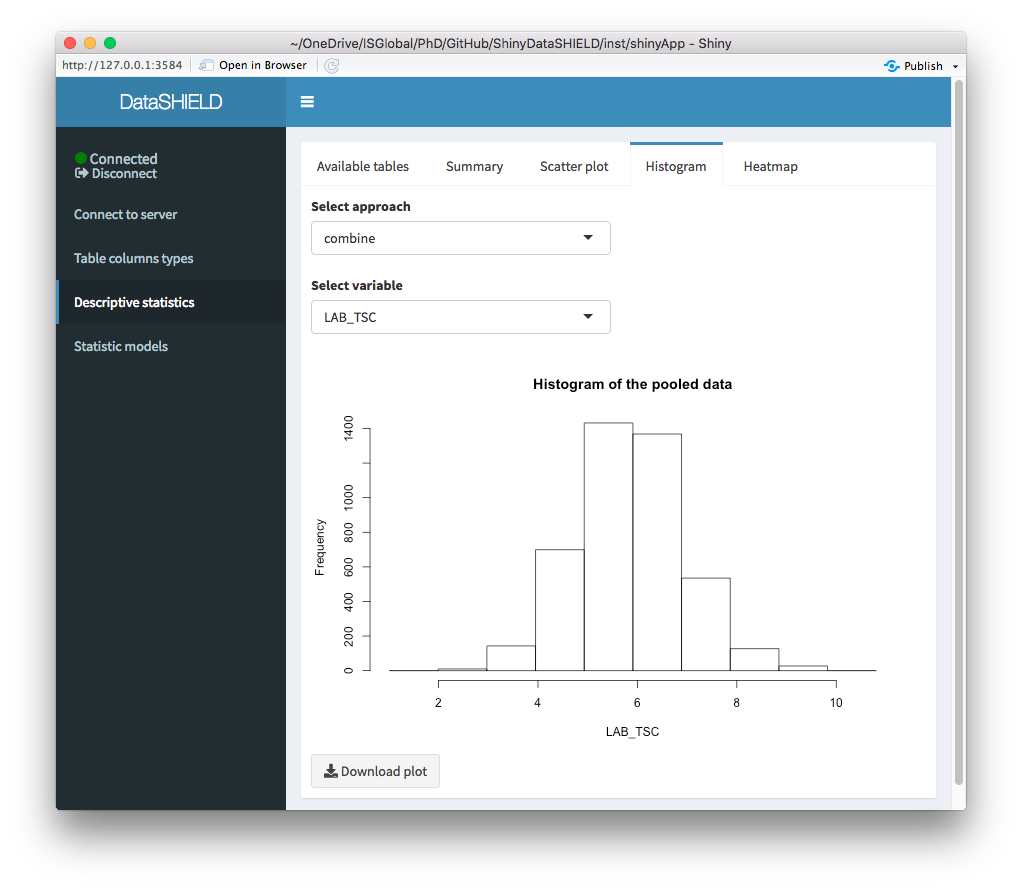
\includegraphics{images/descriptive_stats4.png}

\hypertarget{heatmap}{%
\subsection{Heatmap}\label{heatmap}}

Create a non-disclosive heatmap plot by selecting two numerical variables (one for each axis). There's the option of obtaining a pooled data plot or a different plot for each study server. The selected variables have to be numerial, otherwise the plot is not displayed and a warning message appears.

The dowload plot button saves the shown figure as a \texttt{*.png}.

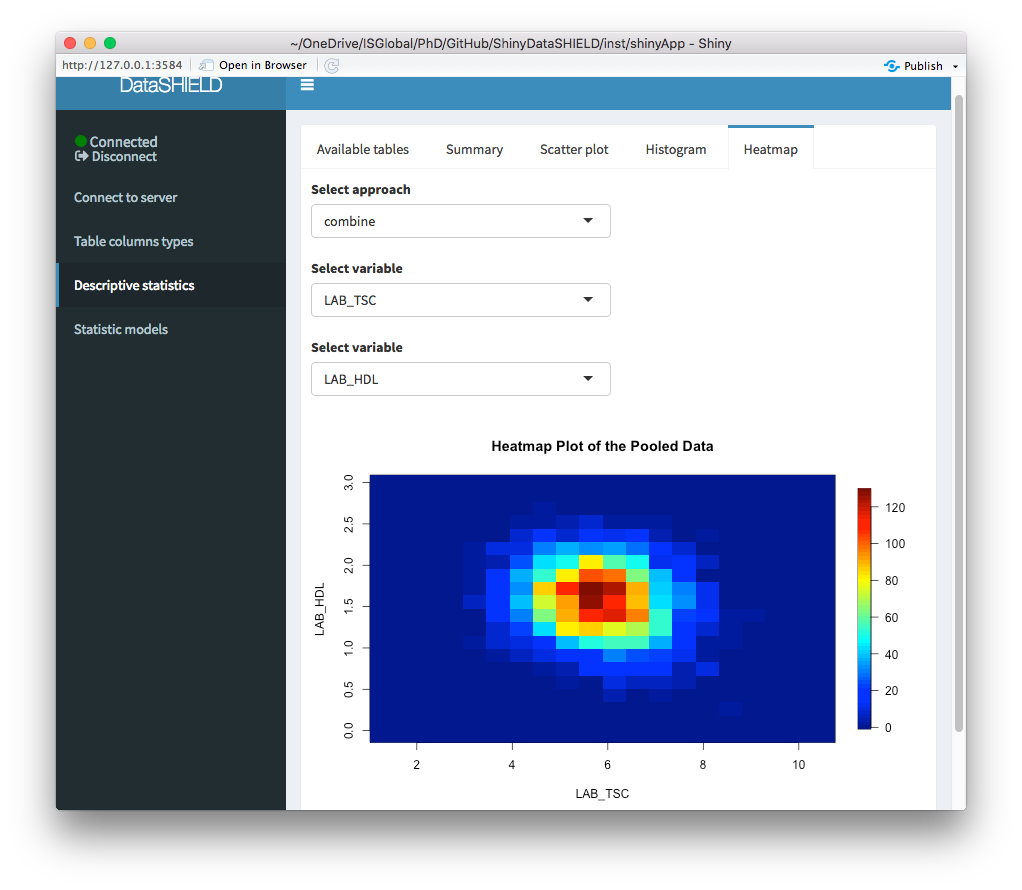
\includegraphics{images/descriptive_stats5.png}

\hypertarget{statistic-models}{%
\section{Statistic models}\label{statistic-models}}

Statistic models are available for tables as well as the following resource types:

\begin{itemize}
\tightlist
\item
  SQL tables
\item
  Tidy data files (tables): \texttt{*.csv}, \texttt{*.tsv}, etc
\end{itemize}

There are two different statisticals models available to fit, GLM models (Statistics models tab) and GLMer models (Mixed statistical models tab).

\hypertarget{glm-models}{%
\subsection{GLM models}\label{glm-models}}

The tab to fit a non-disclosive generalized linear models (GLM) contains a box to manually input the formula, a selector for the output family and a table displaying the variables of the data and the type of each variable. The possible output families are:

\begin{itemize}
\tightlist
\item
  Gaussian
\item
  Poisson
\item
  Binomial
\end{itemize}

There's some help built into ShinyDataSHIELD regarding how to write the GLM formula, which is prompted to the user when clicking on the ``Formula input help'' button. The display of the variables can be toggled on and off for the convenience of use.

Once the GLM model is fitted a table below the variables display will be rendered with the model results. The download button will prompt a system window to select where to store the shown table, it will save it as a \texttt{*.csv}.

When using pooled data, the results of the GLM model will be of the combined data.

(To do: Display more information of why a model fitment fails)

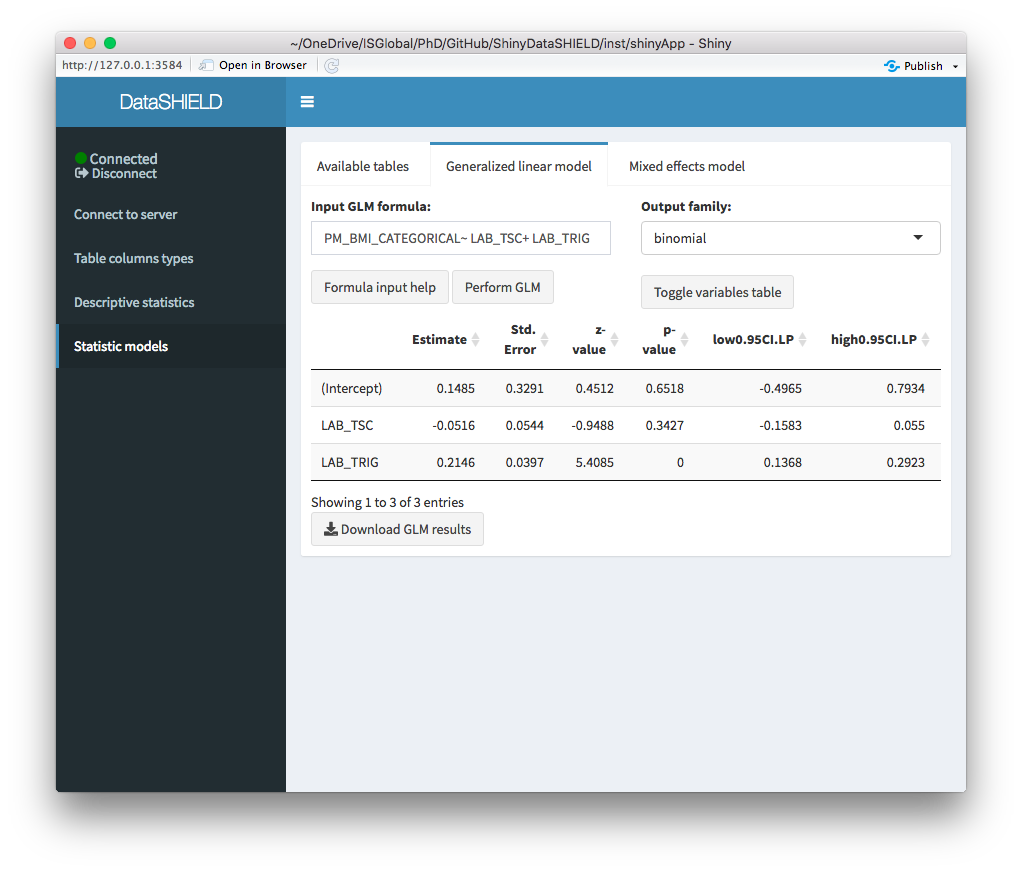
\includegraphics{images/stat_models1.png}

\hypertarget{mixed-models}{%
\subsection{Mixed models}\label{mixed-models}}

The tab to fit non-disclosive generalized mixed effects models (GLMer) contains a box to manually input the formula, a selector for the output family and a table displaying the variables of the data and the type of each variable. The possible output families are:

\begin{itemize}
\tightlist
\item
  Poisson
\item
  Binomial
\end{itemize}

There's some help built into ShinyDataSHIELD regarding how to write the GLMer formula, which is prompted to the user when clicking on the ``Formula input help'' button. The display of the variables can be toggled on and off for the convenience of use.

Once the GLMer model is fitted a table below the variables display will be rendered displaying the results. The download button will prompt a system window to select where to store the shown table, it will save them as a \texttt{*.csv}.

The mixed model results are independent for each study server. There's a selector to toggle between the results of the different study servers.

(To do: Display more information of why a model fitment fails)

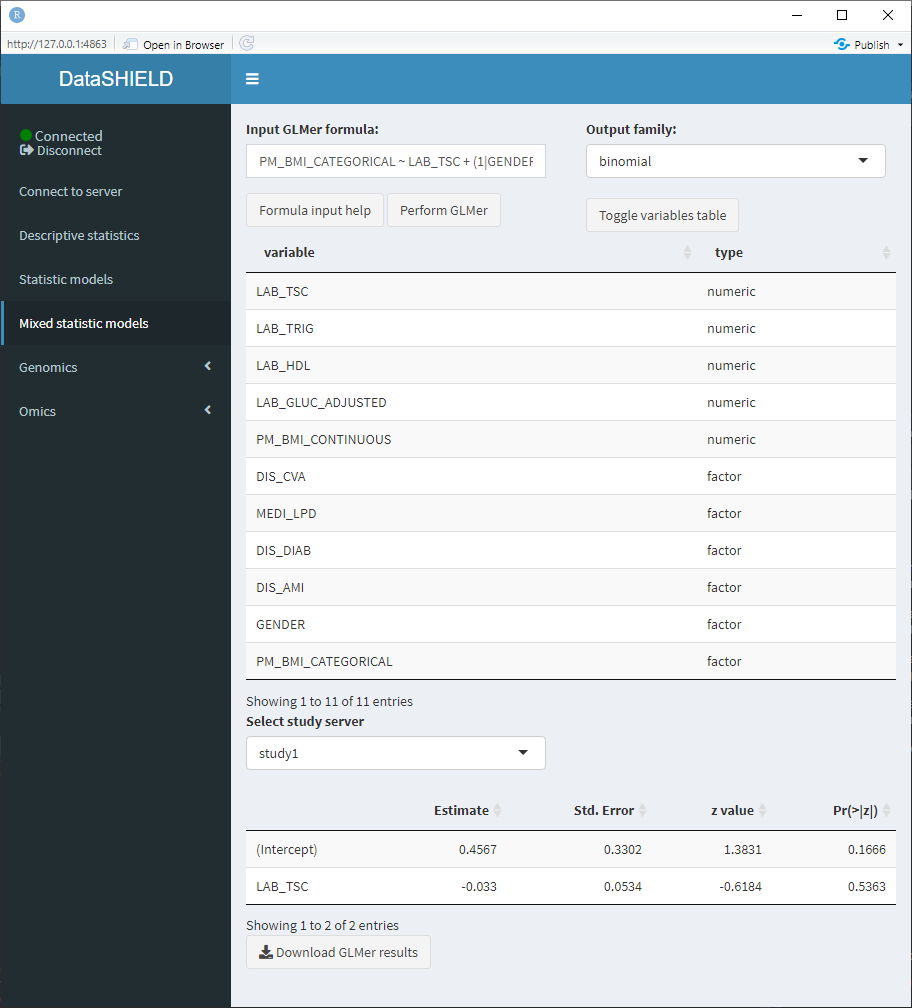
\includegraphics{images/stat_models2.png}

\hypertarget{genomics}{%
\section{Genomics}\label{genomics}}

Inside the genomics tab of dsOmicshiny there are two subtabs, one to perform analysis using BioConductor methods and another to perform analysis using PLINK methods.

\hypertarget{analysis-with-bioconductor}{%
\subsection{Analysis with BioConductor}\label{analysis-with-bioconductor}}

To perform non-disclosive genomic analysis using BioConductor methodologies, the user has to input a VCF resource with a covariates resource (table) on the same study.

When performing this kind of analysis, as explained on the Data Entry section, only one study server can be used.

The Analysis with BioConductor has two sub-tabs, the first one corresponds to the GWAS, and as the name implies is used to perform a GWAS (Genome wide association study) non-disclosive analysis on the loaded data. There is a selector for the condition and the covariates to adjusted for. The fitted model is: snp \textasciitilde{} condition + covar1 + \ldots{} + covarN. The results of the model appear on a table below the selectors. The download button will prompt a system window to select where to store the shown table, it will save it as a \texttt{*.csv}. The second subtab is to display a Manhattan plot of the GWAS results. The dowload plot button saves the shown figure as a \texttt{*.png}.

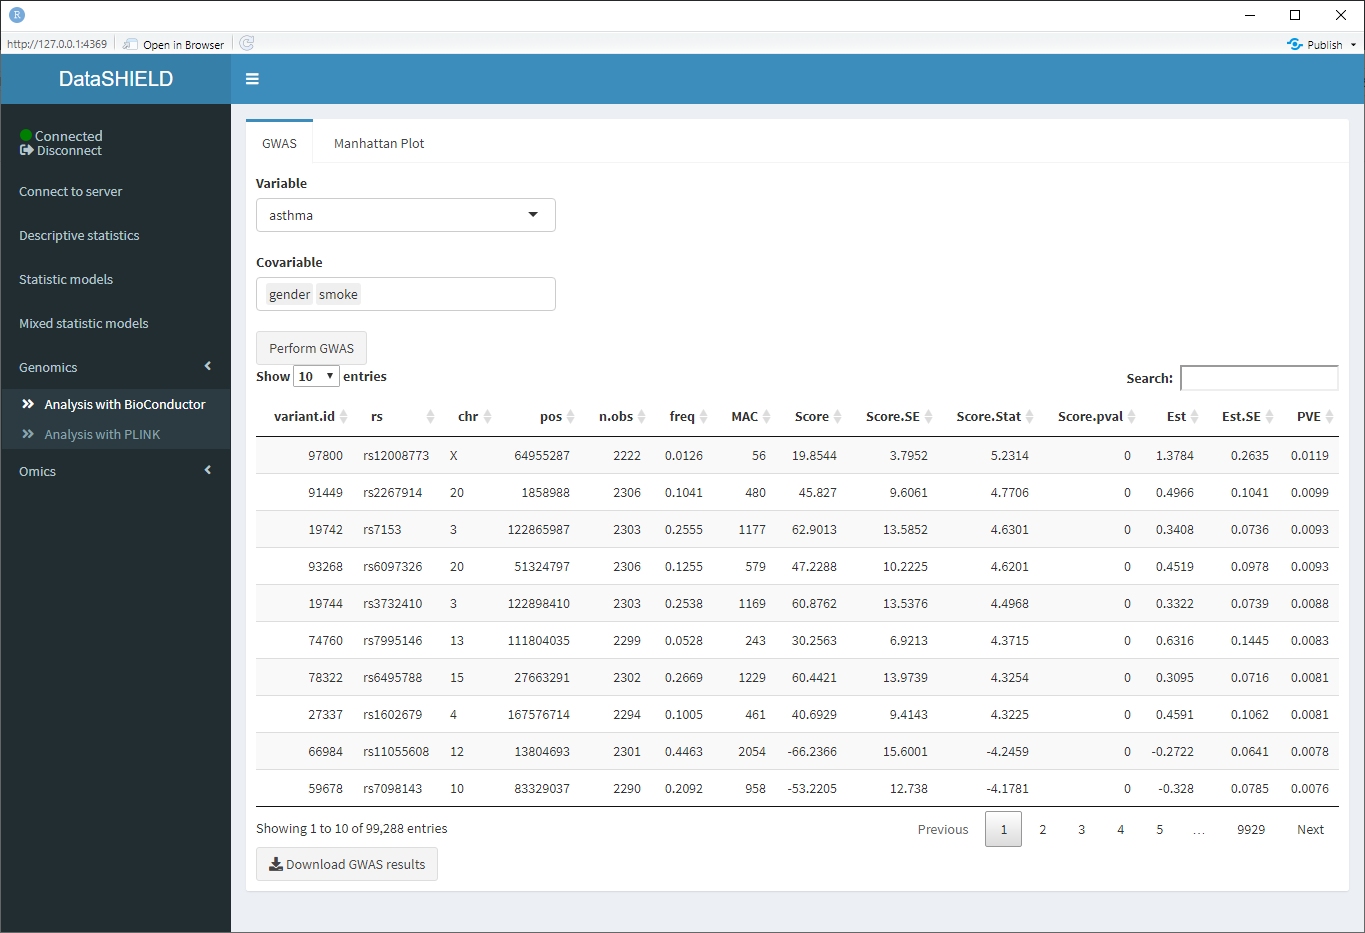
\includegraphics{images/genomics1.png}

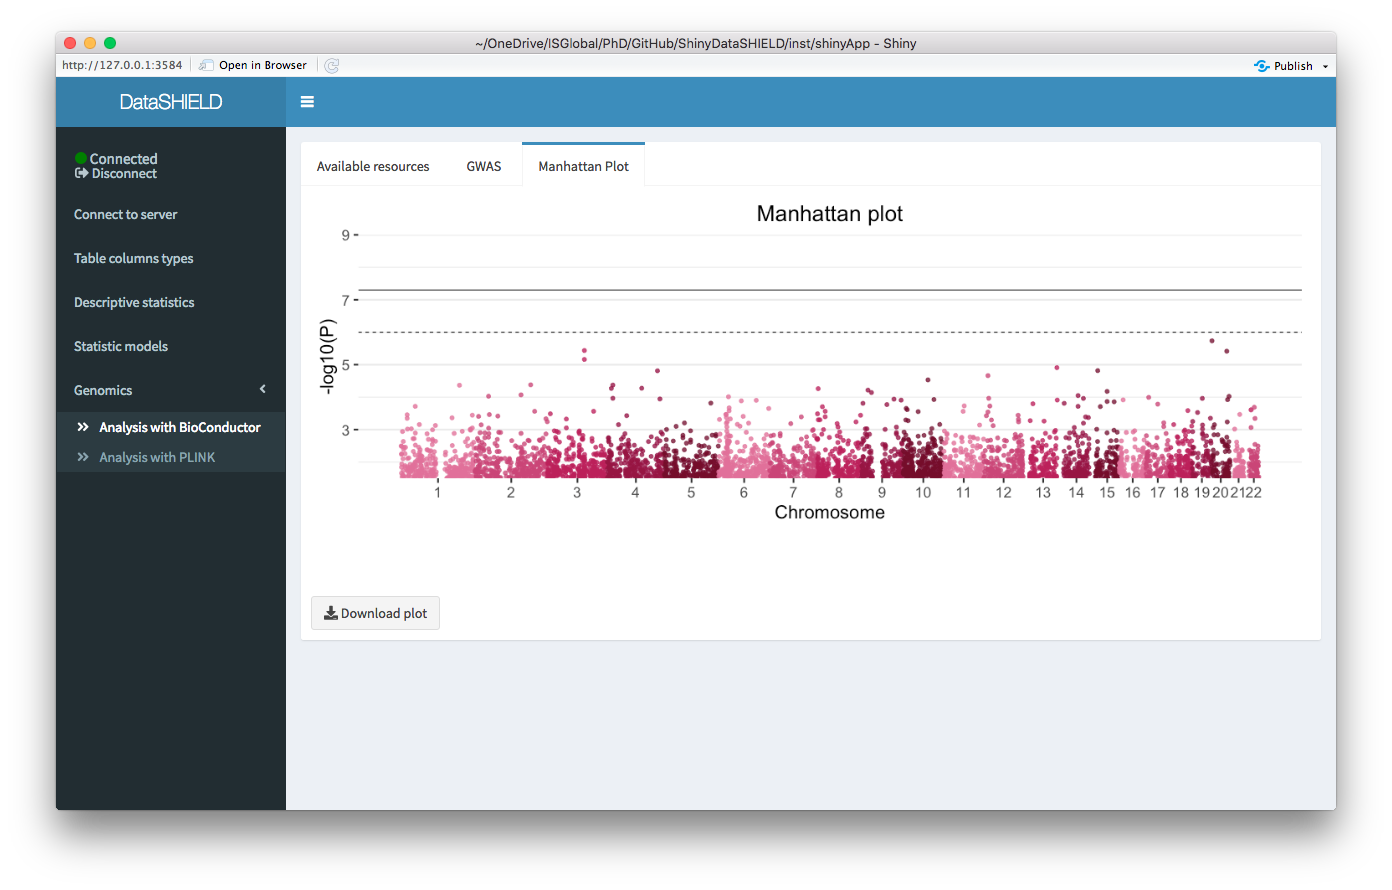
\includegraphics{images/genomics2.png}

\hypertarget{analysis-with-plink}{%
\subsection{Analysis with PLINK}\label{analysis-with-plink}}

To perform non-disclosive analysis using \href{http://zzz.bwh.harvard.edu/plink/index.shtml}{PLINK} commands, the user has to load a SSH resource. The tab contains a field to input the PLINK command and a brief memo stating that when inputing the PLINK command to run there is no need of inputting it as \texttt{plink\ ...} as would be done on a terminal interface, the user has to input just the \texttt{...}; also, there is no need to put \texttt{–out} to indicate the output file.

Once the command is run, a table with the results is displayed under the command input, the download button will prompt a system window to select where to store the shown table, it will save them as a \texttt{*.csv}. A button to display the raw terminal output appears to display the user on a popup the plain text.

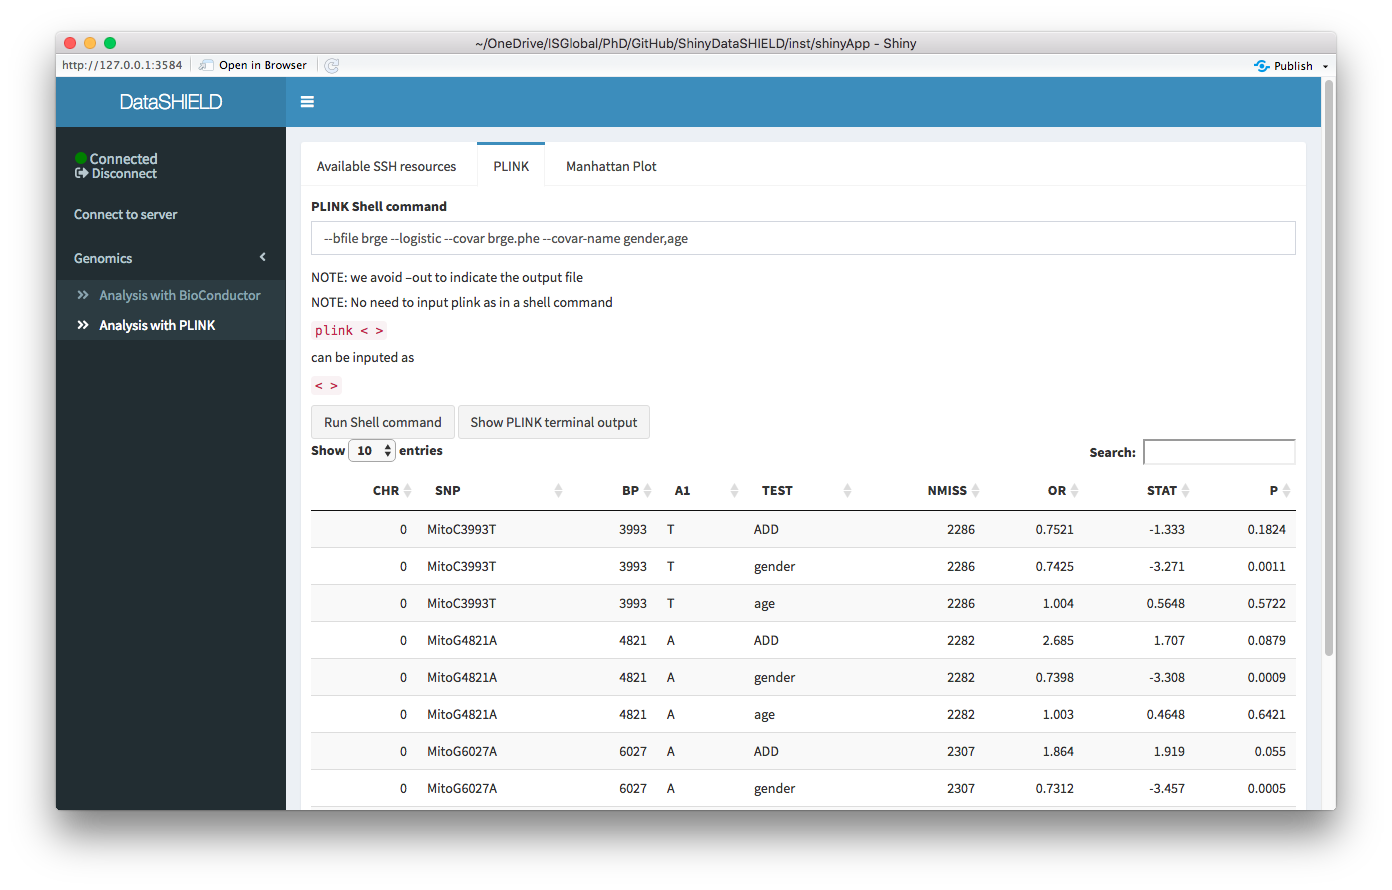
\includegraphics{images/genomics3.png}

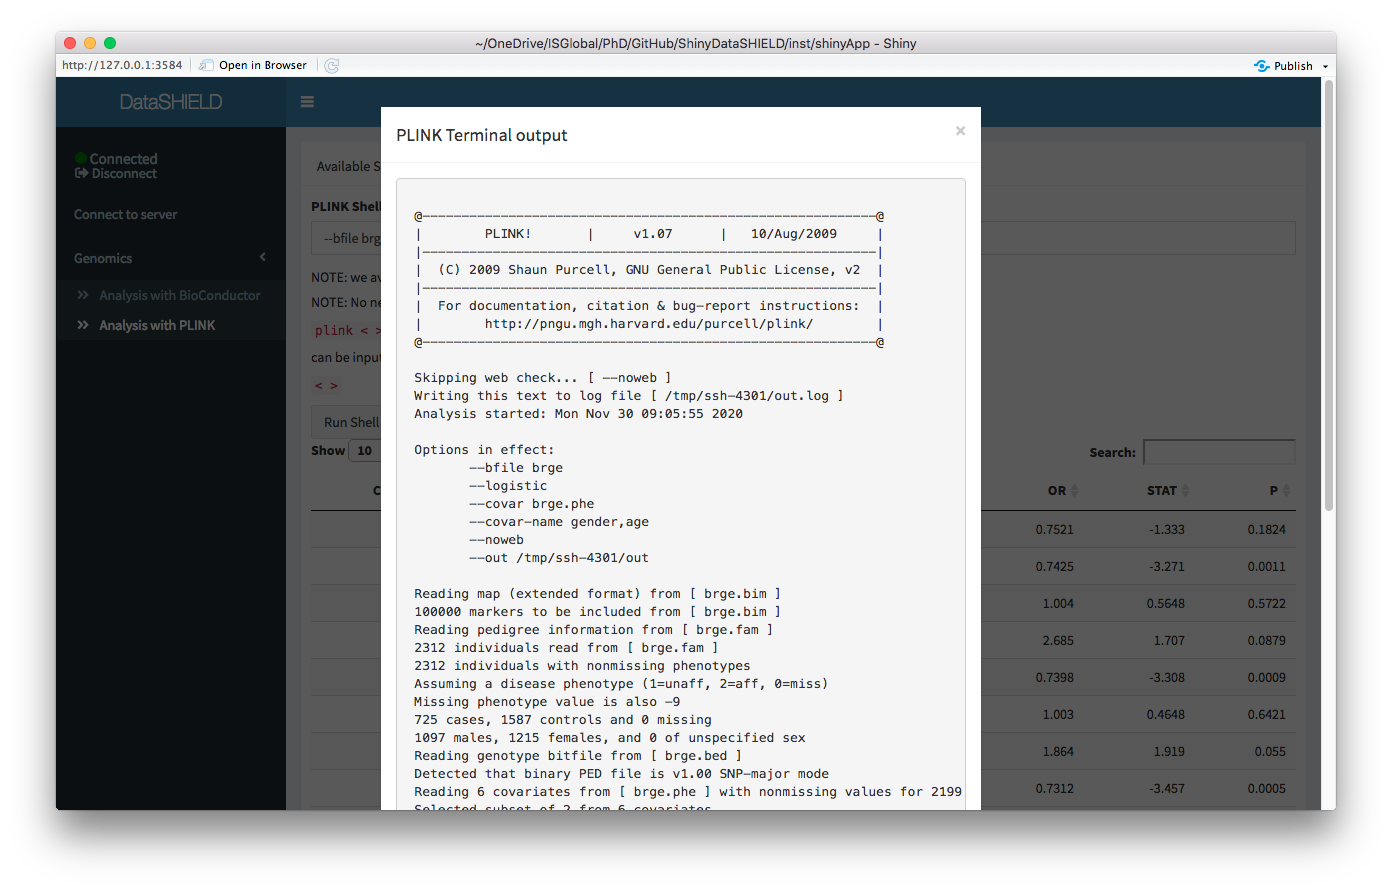
\includegraphics{images/genomics4.png}

There's also a sub-tab to show a Manhattan plot with the results obtained. The dowload plot button saves the shown figure as a \texttt{*.png}.

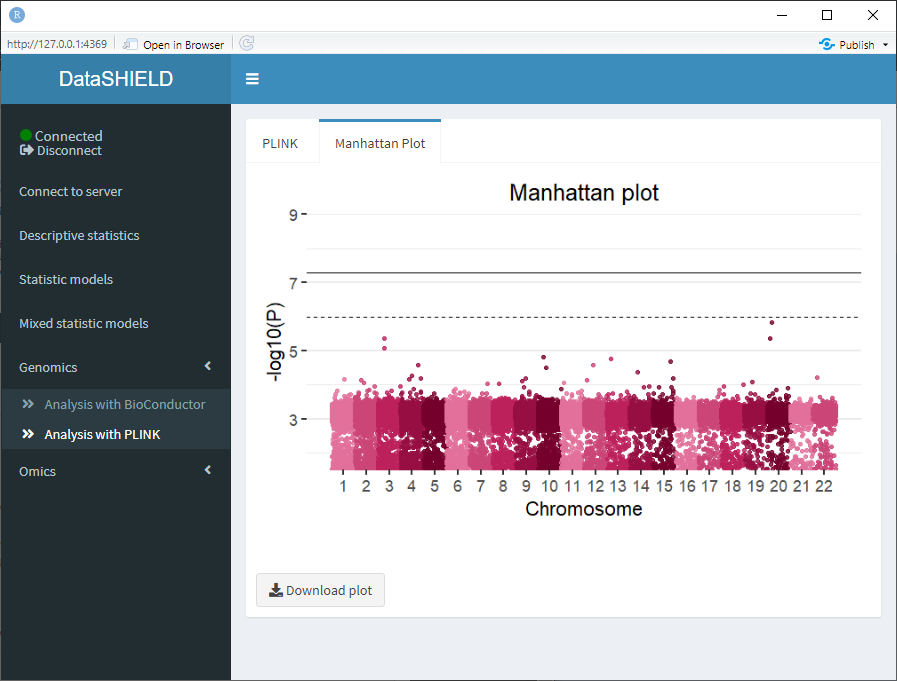
\includegraphics{images/genomics5.png}

\hypertarget{omics}{%
\section{Omics}\label{omics}}

On the Omics tab there are three different subtabs for different methodologies to perform non-disclosive analysis: limma, DESeq and edgeR. The resources that can be used are ExpressionSets and RangegSummarizedExperiments. If the resources are pooled the user has to input each one in a different study on the data entry.

\hypertarget{limma}{%
\subsection{LIMMA}\label{limma}}

The limma non-disclosive analysis tab contains two selectors to select the condition and covariables of the analysis (resulting formula is: feature \textasciitilde{} condition + covar1 + \ldots{} + covarN), there's also a selector to input the annotations columns desired on the output of the analysis. Finally, there's a selector to indicate the type of data that is being studied, whether is microarray or RNAseq. There's a selector to choose to do a surrogate variable analysis.

Once the analysis is performed a table with the results is displayed below the parameter selectors. The download button will prompt a system window to select where to store the shown table, it will save them as a \texttt{*.csv}.

If the analysis is being performed usging a pooled dataset, the shown table corresponds to all the pooled data.

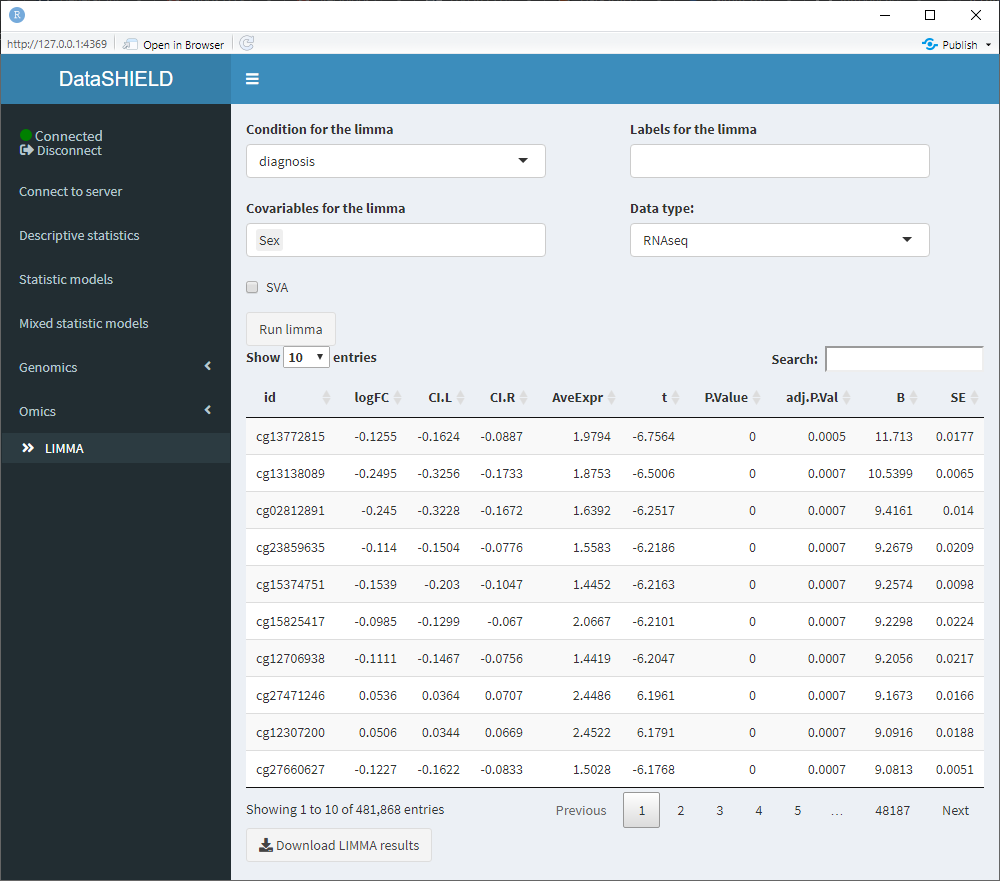
\includegraphics{images/omics1.png}

\hypertarget{deseq}{%
\subsection{DESeq}\label{deseq}}

\hypertarget{edger}{%
\subsection{edgeR}\label{edger}}

\hypertarget{developers-guide}{%
\chapter{Developers Guide}\label{developers-guide}}

Along this section, documentation for future developers and maintainers of ShinyDataSHIELD is provided. It contains information about how the whole Shiny application is structured, all the different scripts that contains, flowcharts of the different files and information on how to extend the capabilities of ShinyDataSHIELD to new types of resources as well as new methodologies.

\begin{longtable}[]{@{}l@{}}
\toprule
\begin{minipage}[b]{0.97\columnwidth}\raggedright
❗ Observation\strut
\end{minipage}\tabularnewline
\midrule
\endhead
\begin{minipage}[t]{0.97\columnwidth}\raggedright
Please read this documentation with the actual source code on the side for easier understanding.\strut
\end{minipage}\tabularnewline
\bottomrule
\end{longtable}

\hypertarget{file-structure-of-shinydatashield}{%
\section{File structure of ShinyDataSHIELD}\label{file-structure-of-shinydatashield}}

Typically Shiny applications are contained in a single file or two files, since the typical structure of a Shiny application is to have a \texttt{server} function and a \texttt{ui} function that can be on the same file or split for larger applications. On dsOmicShiny the \texttt{server} function has been split into different scripts where all of them contains the code of a certain block of the application. It has been done this way to not have a really long \texttt{server} file that is difficult to navigate and debug. There is no need to split the \texttt{ui} file into different scripts since it only contains the graphical declarations of the applications and is really easy to update and navigate.

The different scripts that compose the whole ShinyDataSHIELD are the following:

\begin{itemize}
\tightlist
\item
  \texttt{ui.R}
\item
  \texttt{server.R}, composed of the folowing scripts:

  \begin{itemize}
  \tightlist
  \item
    \texttt{connection.R}
  \item
    \texttt{descriptive\_stats.R}
  \item
    \texttt{download\_handlers.R}
  \item
    \texttt{genomics.R}
  \item
    \texttt{omics.R}
  \item
    \texttt{plot\_renders.R}
  \item
    \texttt{statistic\_models.R}
  \item
    \texttt{table\_renders.R}
  \end{itemize}
\end{itemize}

The file \texttt{server.R} exists to source the different files and it also includes some small funcionalities.

Now a file per file explanation will be given with flowcharts (when needed), remarkable bits of code explanations and general remarks. Also, details on how to implement new functionalities will be given when needed.

\hypertarget{ui.r}{%
\subsection{\texorpdfstring{\texttt{ui.R}}{ui.R}}\label{ui.r}}

Inside this file there are all the declarations of how the graphical user interface (GUI) will look like.

First, it contains a declaration of all the libraries that have to be loaded for the application to run. The libraries are the following: \texttt{DSI,\ DSOpal,\ dsBaseClient,\ dsOmicsClient,\ shinydashboard,\ shiny,\ shinyalert,\ DT,\ data.table,\ shinyjs,\ shinyBS,\ shinycssloaders)}.

The next piece of code found

\begin{Shaded}
\begin{Highlighting}[]
\NormalTok{jscode <-}\StringTok{ '}
\StringTok{$(document).keyup(function(event) \{}
\StringTok{    if ($("#password").is(":focus") && (event.keyCode == 13)) \{}
\StringTok{        $("#connect_server").click();}
\StringTok{    \}}
\StringTok{\});}
\StringTok{'}
\end{Highlighting}
\end{Shaded}

Is a JavaScript declaration that reads as: When the \#password item (corresponds to the text input of the password on the data entry tab) is active (the user is writting in it) and the ``Intro'' key is pressed, trigger the \#connect\_server item (corresponds to the ``Connect'' button on the GUI). That provides the user the typical experience of inputting the login credentials and pressing ``Intro'' to log in.

It's important noting that this is only the declaration of a string with the code inside, to actually make use of it, there is the line 58 of this same file that actually implements it.

\begin{Shaded}
\begin{Highlighting}[]
\NormalTok{tags}\OperatorTok{$}\KeywordTok{head}\NormalTok{(tags}\OperatorTok{$}\KeywordTok{script}\NormalTok{(}\KeywordTok{HTML}\NormalTok{(jscode)))}
\end{Highlighting}
\end{Shaded}

There are a some functions used in this file that are worth mentioning:

\begin{itemize}
\tightlist
\item
  \texttt{hidden()}: From the \texttt{shinyjs} library. The elements wrapped inside of this function will not be rendered by default, they have to be toggled from the server side. Example: A GUI element that needs to be displayed only when a certain condition is met.
\item
  \texttt{withSpinner()}: From the \texttt{shinycssloaders} library. The elements wrapped inside of this function will be displayed as a ``loading spinner'' when they are being processed. This is used to wrap figure displays. Example: A plot that is being rendered, it's better for the user experience to see a ``loading spinner'' so that it knows something is being processed rather than just staring at a blank screen waiting for something to happen.
\item
  \texttt{bsModal()}: From the \texttt{shinyBS} library. It's used to prompt pop-ups to the user. Example: By the click of a button you want to render a pop-up to the application with a figure of an histogram of a selected column of a table.
\end{itemize}

The rest of this file is your average Shiny functions and declarations, read the official \href{https://shiny.rstudio.com/reference/shiny/1.4.0/}{documentation} for any doubts. Please note that ShinyDataSHIELD uses \texttt{shinydashboard} to improve the looks and user experience, for any doubts regarding that please read it's \href{https://rstudio.github.io/shinydashboard/get_started.html}{documentation}.

\hypertarget{server.r}{%
\subsection{\texorpdfstring{\texttt{server.R}}{server.R}}\label{server.r}}

The server file is divided into the following blocks.

\begin{itemize}
\tightlist
\item
  Declaration of reactiveValues: As a code practice measure, all the variables that have to be used in different parts of the code (Example: Table that contains the information about the loaded resources, has to be written when loading the data and afterwards to check whether a resource has been loaded or not) are reactive values. The only occassions where there are ``regular'' variables are inside functions that use variables as placeholders to be used only inside of that function (Example: Storing the results of a middle ground operation to be later used inside the same function to perform the final analysis, whose results will be saved on a reactive value variable). Developers used to lower level languages can see this as \texttt{public} and \texttt{private} variables.
\item
  Sourcing of scripts: Sourcing all the different scripts that actually make up \texttt{server.R}. As said before this is done this way to have a more structured application where each script takes care of a certain block of the application.
\item
  Function declaration: Declaration of a function that given a column of a data table will truncate the decimal places to 4, it's used when rendering tables to not have tables with 9 decimals that look hideous.
\item
  Functions to manage the ``Connected'' / ``No connection'' display. It's a bunch of logic and CSS to just control a small element of the GUI. Basically if the variable \texttt{connection\$active} is \texttt{TRUE} the GUI will show ``Connected'' next to a green dot with a ``Disconnect'' button, otherwise it will display ``No connection'' next to a red dot. When the button ``Disconnect'' is pressed, the function to log out of the server is triggered and the \texttt{connection\$active} variable is set to false.
\end{itemize}


\includegraphics{images/dev1.png}


\includegraphics{images/dev2.png}

The scripts sourced for by the \texttt{server.R} are the following:

\hypertarget{connection.r}{%
\subsubsection{\texorpdfstring{\texttt{connection.R}}{connection.R}}\label{connection.r}}

This is probably the most important script of the whole application, as it's the one that puts some constraints on the capabilities of the application. It also is responsible for loading the data in a proper way in order to ensure that the application capabilities can be extended in the future painlessly (modular).

Inside this script there are five different sections that are triggered by different actions:

\begin{itemize}
\tightlist
\item
  Connection to the server to obtain the projects and resources. Triggered by the button with label ``connect\_server''.
\item
  Get tables / resources from the selected project. Triggered everytime the selector with label ``project\_selected'' is changed.
\item
  Add a study. Triggered by the button with label ``add\_server''.
\item
  Remove a study. Triggered by the button with label ``remove\_server''.
\item
  Load the selected studies to the study servers. Triggered by the button with label ``connect\_selected''.
\end{itemize}

Since it's very important to understand how the code is working in this script, some flowcharts have been created to be read along the code itself and easily understand what's going on.

\begin{longtable}[]{@{}l@{}}
\toprule
\begin{minipage}[b]{0.97\columnwidth}\raggedright
❗ Observation\strut
\end{minipage}\tabularnewline
\midrule
\endhead
\begin{minipage}[t]{0.97\columnwidth}\raggedright
Click on the flowcharts to open them on a separate tab in full-resolution.\strut
\end{minipage}\tabularnewline
\bottomrule
\end{longtable}

There are various red boxes stating some assumptions and some red boxes that show how to implement new features. Let's start by reviewing the assumptions:

\begin{itemize}
\tightlist
\item
  Assumption: Only tables or resources are selected for a study, never both combined
\item
  Assumption: Always only one table per study
\item
  Assumption: Consistency of columns between all the tables of the different studies (pooled data)
\item
  Assumption: A single study can contain multiple resources, multiple studies can only contain one resource per study
\end{itemize}

All the assumptions boxes are located on the parts of the flowchart that would have to be modified in order to change them.

When loading the selected resources or tables into the study servers, the table \texttt{available\_tables} is created. The name is a little bit confusing since it actually contains the information about tables and resources, the developer apologizes as this variable was set at the beginning of the development and has not been updated. Nevertheless, it's an important variable of the application, the structure of this table is the following.

\begin{longtable}[]{@{}l@{}}
\toprule
\begin{minipage}[b]{0.97\columnwidth}\raggedright
❗ Observation\strut
\end{minipage}\tabularnewline
\midrule
\endhead
\begin{minipage}[t]{0.97\columnwidth}\raggedright
On the following table there are code examples, it is marked as \texttt{THIS} wherever the column value would be placed.\strut
\end{minipage}\tabularnewline
\bottomrule
\end{longtable}

\begin{longtable}[]{@{}ll@{}}
\toprule
\begin{minipage}[b]{0.07\columnwidth}\raggedright
Column\strut
\end{minipage} & \begin{minipage}[b]{0.87\columnwidth}\raggedright
Description\strut
\end{minipage}\tabularnewline
\midrule
\endhead
\begin{minipage}[t]{0.07\columnwidth}\raggedright
server\strut
\end{minipage} & \begin{minipage}[t]{0.87\columnwidth}\raggedright
Contains the names of the study servers.\texttt{connection\$builder\$append(server\ =\ THIS,\ url\ =\ input\$url,\ \ \ \ \ \ \ \ \ \ \ \ \ \ \ \ \ \ \ \ \ \ \ \ \ \ \ \ \ \ \ \ \ \ user\ =\ input\$user,\ password\ =\ input\$password,\ driver\ =\ "OpalDriver")}\strut
\end{minipage}\tabularnewline
\begin{minipage}[t]{0.07\columnwidth}\raggedright
table\strut
\end{minipage} & \begin{minipage}[t]{0.87\columnwidth}\raggedright
Name of the table in the Opal server. Structure: \texttt{project\_name.table\_name}\strut
\end{minipage}\tabularnewline
\begin{minipage}[t]{0.07\columnwidth}\raggedright
table\_internal\strut
\end{minipage} & \begin{minipage}[t]{0.87\columnwidth}\raggedright
Name assigned to the table on the study server. Assigned by:\texttt{datashield.assign.table(THIS,\ table)}\strut
\end{minipage}\tabularnewline
\begin{minipage}[t]{0.07\columnwidth}\raggedright
type\_resource\strut
\end{minipage} & \begin{minipage}[t]{0.87\columnwidth}\raggedright
Type of the resource\strut
\end{minipage}\tabularnewline
\begin{minipage}[t]{0.07\columnwidth}\raggedright
resource\strut
\end{minipage} & \begin{minipage}[t]{0.87\columnwidth}\raggedright
Name of the resource in the Opal server. Structure: \texttt{project\_name.resource\_name}\strut
\end{minipage}\tabularnewline
\begin{minipage}[t]{0.07\columnwidth}\raggedright
resource\_internal\strut
\end{minipage} & \begin{minipage}[t]{0.87\columnwidth}\raggedright
Name assigned to the resource on the study server. Assigned by:\texttt{datashield.assign.resource(THIS,\ resource)}\strut
\end{minipage}\tabularnewline
\bottomrule
\end{longtable}

The Opal server can host different types of resources, to name a few there are \texttt{ExpressionSet}, \texttt{RangedSummarizedExperiment} and \texttt{SQLResourceClient}. Each type of resource needs a special treatment to be used, for example \texttt{SQLResourceClient} resources are plain tables, so they need to be converted to tables on the study server to use them. Currently the following resource types are supported by ShinyDataSHIELD.

\begin{longtable}[]{@{}lll@{}}
\toprule
\begin{minipage}[b]{0.16\columnwidth}\raggedright
Resource type\strut
\end{minipage} & \begin{minipage}[b]{0.56\columnwidth}\raggedright
Treatment\strut
\end{minipage} & \begin{minipage}[b]{0.19\columnwidth}\raggedright
Name of the resource type on \texttt{available\_tables}\strut
\end{minipage}\tabularnewline
\midrule
\endhead
\begin{minipage}[t]{0.16\columnwidth}\raggedright
TidyFileResourceClient, SQLResourceClient\strut
\end{minipage} & \begin{minipage}[t]{0.56\columnwidth}\raggedright
- \texttt{as.resource.data.frame(resource)}- Change name to \texttt{table1} instead of \texttt{resource1}- Get column names (\texttt{table\_columns}) and types (\texttt{table\_columns\_types}) and save them\strut
\end{minipage} & \begin{minipage}[t]{0.19\columnwidth}\raggedright
\texttt{table}\strut
\end{minipage}\tabularnewline
\begin{minipage}[t]{0.16\columnwidth}\raggedright
SshResourceClient\strut
\end{minipage} & \begin{minipage}[t]{0.56\columnwidth}\raggedright
No treatment\strut
\end{minipage} & \begin{minipage}[t]{0.19\columnwidth}\raggedright
\texttt{ssh}\strut
\end{minipage}\tabularnewline
\begin{minipage}[t]{0.16\columnwidth}\raggedright
GdsGenotypeReader\strut
\end{minipage} & \begin{minipage}[t]{0.56\columnwidth}\raggedright
- \texttt{as.resource.object(resource)}\strut
\end{minipage} & \begin{minipage}[t]{0.19\columnwidth}\raggedright
\texttt{r\_obj\_vcf}\strut
\end{minipage}\tabularnewline
\begin{minipage}[t]{0.16\columnwidth}\raggedright
ExpressionSet\strut
\end{minipage} & \begin{minipage}[t]{0.56\columnwidth}\raggedright
- \texttt{as.resource.object(resource)}- Copy as \texttt{table1} to use the descriptive statistics tab with this resource\strut
\end{minipage} & \begin{minipage}[t]{0.19\columnwidth}\raggedright
\texttt{r\_obj\_eset}\strut
\end{minipage}\tabularnewline
\begin{minipage}[t]{0.16\columnwidth}\raggedright
RangedSummarizedExperiment\strut
\end{minipage} & \begin{minipage}[t]{0.56\columnwidth}\raggedright
- \texttt{as.resource.object(resource)}- Copy as \texttt{table1} to use the descriptive statistics tab with this resource\strut
\end{minipage} & \begin{minipage}[t]{0.19\columnwidth}\raggedright
\texttt{r\_obj\_rse}\strut
\end{minipage}\tabularnewline
\begin{minipage}[t]{0.16\columnwidth}\raggedright
Any other resource type\strut
\end{minipage} & \begin{minipage}[t]{0.56\columnwidth}\raggedright
- \texttt{as.resource.object(resource)}\strut
\end{minipage} & \begin{minipage}[t]{0.19\columnwidth}\raggedright
\texttt{r\_obj}\strut
\end{minipage}\tabularnewline
\bottomrule
\end{longtable}

Examples of \texttt{available\_tables} depending on the selected resources and study servers.

\begin{itemize}
\tightlist
\item
  A pooled study of three tables, each one on a different study server:
\end{itemize}

\begin{longtable}[]{@{}llll@{}}
\toprule
server & table & table\_internal & type\_resource\tabularnewline
\midrule
\endhead
server1 & CNSIM.CNSIM1 & table1 & table\tabularnewline
server2 & CNSIM.CNSIM2 & table1 & table\tabularnewline
server3 & CNSIM.CNSIM3 & table1 & table\tabularnewline
\bottomrule
\end{longtable}

What can be seen from this table is that there are three study servers and each one contains a different table. Since they are located on different servers they have the same internal names.

\begin{itemize}
\tightlist
\item
  A pooled study using resources that contain ExpressionSets
\end{itemize}

\begin{longtable}[]{@{}llll@{}}
\toprule
server & resource & resource\_internal & type\_resource\tabularnewline
\midrule
\endhead
server1 & RSRC.GSE66351\_1 & resource1 & r\_obj\_eset\tabularnewline
server2 & RSRC.GSE66351\_2 & resource1 & r\_obj\_eset\tabularnewline
\bottomrule
\end{longtable}

We can observe the same things as the previous case but here we have a different \texttt{type\_resource}

\begin{itemize}
\tightlist
\item
  Single study server with two resources (one of which is actually a table)
\end{itemize}

\begin{longtable}[]{@{}llllll@{}}
\toprule
server & resource & resource\_internal & type\_resource & table & table\_internal\tabularnewline
\midrule
\endhead
server1 & RS.G\_covars & resource1 & table & RS.G\_covars & table1\tabularnewline
server1 & RS.G\_vcf & resource2 & r\_obj\_vcf & NA & NA\tabularnewline
\bottomrule
\end{longtable}

On this case we can see that there are two resources on the same server, and the resource of type table is actually copied into a new variable (internal) with the name \texttt{table1}.

Now, let's look at some examples to add new resource types on the \texttt{connection.R} file. There are different cases for the treatment that the new resource requires.

\begin{itemize}
\tightlist
\item
  Resources that contain tables. They have to be treated as so in order to be able to use them on the ``Descriprive statistics'', if a new type of resource that contains tables is being implemented, change line 88 \texttt{if\ (any(c("TidyFileResourceClient",\ "SQLResourceClient")\ \%in\%\ resource\_type))\{}, in this line we would add the name of the new resource type that is going to be treated as a table. Example: A new resource called \texttt{NewTables} is being introduced, the line 88 has to be changed to \texttt{if\ (any(c("TidyFileResourceClient",\ "SQLResourceClient",\ "NewTables")\ \%in\%\ resource\_type))\{}.
\item
  Resources that just need to be loaded with no further action performed to them. Add another \texttt{else\ if} statement after line 107. Example: New resource called \texttt{Simple\_resource}
\end{itemize}

\begin{Shaded}
\begin{Highlighting}[]
\ControlFlowTok{else} \ControlFlowTok{if}\NormalTok{ (}\StringTok{"Simple_resource"} \OperatorTok\StringTok{ }\NormalTok{resource_type)\{}
            \CommentTok{# Update available_tables list with the new resource type name}
\NormalTok{            lists}\OperatorTok{$}\NormalTok{available_tables <-}\StringTok{ }\NormalTok{lists}\OperatorTok{$}\NormalTok{available_tables[resource_internal }\OperatorTok{==}\StringTok{ }\KeywordTok{paste0}\NormalTok{(}\StringTok{"resource"}\NormalTok{, i), type_resource }\OperatorTok{:}\ErrorTok{=}\StringTok{ "simple_resource"}\NormalTok{]}
\NormalTok{          \}}
\end{Highlighting}
\end{Shaded}

\begin{itemize}
\tightlist
\item
  Resources that need to be converted into R objects (\texttt{datashield.assign.expr(conns,\ symbol\ =\ "methy",\ expr\ =\ quote(as.resource.object(res)))}) and nothing else. Will work out of the box (the \texttt{type\_resource} column of the \texttt{lists\$available\_tables} table will read \texttt{r\_obj}).
\item
  Resources that need to be converted into R objects (\texttt{datashield.assign.expr(conns,\ symbol\ =\ "methy",\ expr\ =\ quote(as.resource.object(res)))}) and be further processed. Add another \texttt{else\ if} statement after line 135. Example: A new type of resource called \texttt{special\_resource} that contains some variable names that are desired to be saved on a variable to feed a list on the GUI.
\end{itemize}

\begin{Shaded}
\begin{Highlighting}[]
\ControlFlowTok{else} \ControlFlowTok{if}\NormalTok{(}\StringTok{"special_resource"} \OperatorTok\StringTok{ }\NormalTok{resource_type) \{}
              \CommentTok{# Update available_tables list with the new resource type name}
\NormalTok{              lists}\OperatorTok{$}\NormalTok{available_tables <-}\StringTok{ }\NormalTok{lists}\OperatorTok{$}\NormalTok{available_tables[resource_internal }\OperatorTok{==}\StringTok{ }\KeywordTok{paste0}\NormalTok{(}\StringTok{"resource"}\NormalTok{, i), type_resource }\OperatorTok{:}\ErrorTok{=}\StringTok{ "special_resource"}\NormalTok{]}
              \CommentTok{# Perform the needed actions for this resource, on this example: using the ds.varLabels function}
              \CommentTok{# and save the output on a variable}
\NormalTok{              lists}\OperatorTok{$}\NormalTok{table_columns <-}\StringTok{ }\KeywordTok{ds.varLabels}\NormalTok{(}\KeywordTok{paste0}\NormalTok{(}\StringTok{"resource"}\NormalTok{, i), }\DataTypeTok{datasources =}\NormalTok{ connection}\OperatorTok{$}\NormalTok{conns)}\OperatorTok{$}\NormalTok{server1}
\NormalTok{            \}}
\end{Highlighting}
\end{Shaded}

There's already a variable called \texttt{table\_columns} for those types of cases. If the new resource requires novel things just update the variables on the top of the \texttt{server.R} and apply the required methodologies.

As a summary, \texttt{connection.R} loads the selected tables / resources into the study servers and updates the table \texttt{available\_tables} with the information about the loaded resources / tables and their types. The idea is that when X resource is loaded, it's already processed on the \texttt{connection.R} to be used on a certain block, so all the funcional blocks only contain the code of their core functionality, not code to pre-process the resource before analyzing it.

\hypertarget{descriptive_stats.r}{%
\subsubsection{\texorpdfstring{\texttt{descriptive\_stats.R}}{descriptive\_stats.R}}\label{descriptive_stats.r}}

The script contains all the render functions to render the selectors of the block. This has to be done this way since the ``Variable'' selector for example is fed a list created when inputing the data, so it's a dynamic value. Putting the render functions on the \texttt{ui.R} will result in the application crashing since the list of variables is non existant at the time of launching the Shiny application.

Besides that, there's also an \texttt{observe} function that takes care of warning the user if no connection is active and this tab is selected, as well as warning the user if the resource of the study server is not appropiate for this tab.

This block basically contains figures and tables, and they are actually created on the \texttt{table\_renders.R} and \texttt{plot\_renders.R}.

\hypertarget{statistics_models.r}{%
\subsubsection{\texorpdfstring{\texttt{statistics\_models.R}}{statistics\_models.R}}\label{statistics_models.r}}

This script contains the functions to run two tabs, the ``Statistic models'' and the ``Mixed statistic models''. In this tab there are two sets of very similar triggers (\texttt{observeEvent()}):

\begin{itemize}
\tightlist
\item
  A toggle to show and hide the table that displays the variables of the study table and their types. (\texttt{toggleElement()})
\item
  Perform the model with the inputed data. Encapsulated on a \texttt{tryCatch} so that if there's an error when calculating the model, there's a \texttt{shinyalert()} to prompt a popup warning in the GUI.
\item
  Trigger that displays a \texttt{shinyalert()} popup with some help regarding the input of the formula.
\end{itemize}

Those tree elements are doubled, one for the GLM model and the other for the GLMerSLMA. Note that for the GLMerSLMA there's an extra element to select the study to show the results of, since the GLM provides a model for the pooled data and GLMer outputs the coefficients for each of the study servers.

Besides that, there's also an \texttt{observe} function that takes care of warning the user if no connection is active and this tab is selected, as well as warning the user if the resource of the study server is not appropiate for this tab.

\hypertarget{genomics.r}{%
\subsubsection{\texorpdfstring{\texttt{genomics.R}}{genomics.R}}\label{genomics.r}}

On this scripts there are all the genomics methodologies implemented into ShinyDataSHIELD

\begin{itemize}
\tightlist
\item
  PLINK files: The functions corresponding to the PLINK analysis is just a trigger that reads the inputed command and performs the querry and a \texttt{renderText()} function to render the raw text output from the PLINK.
\item
  VCF files: For this resources, there are the following items

  \begin{itemize}
  \tightlist
  \item
    Render functions for the lists of variables.
  \item
    Trigger to perform the GWAS, encapsulated on a \texttt{tryCatch()} so that if there's an error when calculating the GWAS, there's a \texttt{shinyalert()} to prompt a popup warning in the GUI.
  \end{itemize}
\end{itemize}

It's important noting that when using VCF files the user has to load two files into the study, the VCF and a covariates files (table). The \texttt{connection.R} script handles that and loads the VCF as a resource and the covariates as a table, so on the \texttt{available\_tables} they have their own different \texttt{type\_resource} value. Therefore, this can be done:

\begin{Shaded}
\begin{Highlighting}[]
\NormalTok{x=lists}\OperatorTok{$}\NormalTok{available_tables[type_resource }\OperatorTok{==}\StringTok{ "r_obj_vcf"}\NormalTok{, resource_internal]}
\NormalTok{covars =}\StringTok{ }\NormalTok{lists}\OperatorTok{$}\NormalTok{available_tables[type_resource }\OperatorTok{==}\StringTok{ "table"}\NormalTok{, resource_internal]}
\end{Highlighting}
\end{Shaded}

This assumes that when the user wants to perform this analysis, there's only a single study with two resources, one of type \texttt{table} for the covars and one of type \texttt{r\_obj\_vcf}. It's important noting (assuming that the part of the \texttt{connection.R} has been understood) that a VCF resource is a type of resource that does not need further treatment than being converted to an R object (\texttt{datashield.assign.expr(conns,\ symbol\ =\ "methy",\ expr\ =\ quote(as.resource.object(res)))}) however it was of interest giving it a different \texttt{type\_resource} name than the standard \texttt{r\_obj} that is given to this types of resources, so it has it's own \texttt{else\ if} statement on the \texttt{connection.R}.

Besides that, there's also an \texttt{observe} function that takes care of warning the user if no connection is active and this tab is selected, as well as warning the user if the resource of the study server is not appropiate for either tab (a SSH resource will trigger a warning if the ``Analysis with BioConductor'' tab is selected).

\hypertarget{omics.r}{%
\subsubsection{\texorpdfstring{\texttt{omics.R}}{omics.R}}\label{omics.r}}

This script is virtually the same as the VCF part of the \texttt{genomics.R}, it contains GUI renders, a trigger to perform the analysis itself encapsulated on a \texttt{tryCatch()} and the \texttt{observe} function for good measure. It's important noting that so far it only has implemented LIMMA, on the future it should include DESeq and edgeR methodologies.

\hypertarget{table_renders.r}{%
\subsubsection{\texorpdfstring{\texttt{table\_renders.R}}{table\_renders.R}}\label{table_renders.r}}

This script creates the displays of all the tables of ShinyDataSHIELD, it uses the \texttt{DT} package to do so. Besides the \texttt{descriptive\_summary} table, all the other tables just render results from other functions.

There are some things to point of this script:

\begin{itemize}
\tightlist
\item
  As can be seen in \texttt{descriptive\_summary} table, you can actually perform operations inside of a \texttt{renderDT} function and display the result of them.
\item
  The most used options for the tables aesthetics are the following
\end{itemize}

\begin{Shaded}
\begin{Highlighting}[]
\NormalTok{options=}\KeywordTok{list}\NormalTok{(}\DataTypeTok{columnDefs =} \KeywordTok{list}\NormalTok{(}\KeywordTok{list}\NormalTok{(}\DataTypeTok{visible=}\OtherTok{FALSE}\NormalTok{, }\DataTypeTok{targets=}\KeywordTok{c}\NormalTok{(}\DecValTok{0}\NormalTok{))),}
                                          \DataTypeTok{paging =} \OtherTok{FALSE}\NormalTok{, }\DataTypeTok{searching =} \OtherTok{FALSE}\NormalTok{)}
\end{Highlighting}
\end{Shaded}

This prevents the \texttt{rownames} column to be displayed (usually it just contains the numeration of rows 1\ldots N, be aware sometimes it's of interest to see this column) and eliminates the paging and searching functionalities of the table. For small tables it makes sense to not show that but on big tables those options are set to \texttt{TRUE}, as it's very useful to have a search box on them.

\begin{itemize}
\tightlist
\item
  The tables that display numerical columns (mixed or not with non-numerical columns) are actually passed through the \texttt{format\_num} function (defined on \texttt{server.R}) so the displayed table has only four decimals but the actual table (the one that can be saved) has all the decimals. This is done using the following code
\end{itemize}

\begin{Shaded}
\begin{Highlighting}[]
\KeywordTok{as.data.table}\NormalTok{(}\KeywordTok{lapply}\NormalTok{(}\KeywordTok{as.data.table}\NormalTok{(vcf_results}\OperatorTok{$}\NormalTok{result_table_gwas}\OperatorTok{$}\NormalTok{server1), format_num))}
\end{Highlighting}
\end{Shaded}

This will pass each column to the function and if it's numerical the decimals will be cut to 4.

\begin{itemize}
\tightlist
\item
  The table output structure of the LIMMA results look different than the others, this is because when performing a LIMMA with pooled resources it returns one table for each study, what is being done is just binding them to display to the user all the obtained results.
\end{itemize}

\hypertarget{plot_renders.r}{%
\subsubsection{\texorpdfstring{\texttt{plot\_renders.R}}{plot\_renders.R}}\label{plot_renders.r}}

There are two types of plots on ShinyDataSHIELD, the ones created with the base function \href{https://www.rdocumentation.org/packages/graphics/versions/3.6.2/topics/plot}{plot} and the ones created with the \href{https://ggplot2.tidyverse.org/}{ggplot} library. In order to later recover the plots to download them, they actually have a different structure.

\begin{itemize}
\tightlist
\item
  Base plot structure:
\end{itemize}

\begin{Shaded}
\begin{Highlighting}[]
\NormalTok{output}\OperatorTok{$}\NormalTok{random_plot <-}\StringTok{ }\KeywordTok{renderPlot}\NormalTok{(\{}
\NormalTok{  plots}\OperatorTok{$}\NormalTok{random_plot <-}\StringTok{ }\ControlFlowTok{function}\NormalTok{()\{}
    \KeywordTok{function_that_generates_the_plot_using_base_package}\NormalTok{(arguments)}
\NormalTok{  \}}
\NormalTok{  plots}\OperatorTok{$}\KeywordTok{random_plot}\NormalTok{()}
\NormalTok{\})}
\end{Highlighting}
\end{Shaded}

For the base plots, a function is declared that returns the plot and is called to generate the plot to the GUI.

\begin{itemize}
\tightlist
\item
  Ggplot structure:
\end{itemize}

\begin{Shaded}
\begin{Highlighting}[]
\NormalTok{output}\OperatorTok{$}\NormalTok{manhattan <-}\StringTok{ }\KeywordTok{renderPlot}\NormalTok{(\{}
\NormalTok{  plots}\OperatorTok{$}\NormalTok{ggplot <-}\StringTok{ }\KeywordTok{function_that_generates_the_plot_using_ggplot2_package}\NormalTok{(arguments)}
\NormalTok{  plots}\OperatorTok{$}\NormalTok{ggplot}
\NormalTok{\})}
\end{Highlighting}
\end{Shaded}

In this case the plot is saved, ggplot will generate a plot variable that can be called to render the plot.

On this script there are two plots that are inside a \texttt{renderCachedPlot} function instead of a \texttt{renderPlot} because they take really long to calculate and it's better to cache them.

Inside of the \texttt{renderPlot} function some other code can be put, such as toggles to GUI elements or \texttt{tryCatch()} functions.

\hypertarget{download_handlers.r}{%
\subsubsection{\texorpdfstring{\texttt{download\_handlers.R}}{download\_handlers.R}}\label{download_handlers.r}}

In this script everything related to downloading plots and tables is found. There are basically three types of structures

\begin{itemize}
\tightlist
\item
  Table downloader: To download a \texttt{*csv}. Structure:
\end{itemize}

\begin{Shaded}
\begin{Highlighting}[]
\NormalTok{output}\OperatorTok{$}\NormalTok{table_download <-}\StringTok{ }\KeywordTok{downloadHandler}\NormalTok{(}
  \DataTypeTok{filename =} \StringTok{"table.csv"}\NormalTok{,}
  \DataTypeTok{content =} \ControlFlowTok{function}\NormalTok{(file) \{}
    \KeywordTok{write.csv}\NormalTok{(}
\NormalTok{      variable_that_contains_table}
\NormalTok{      , file, }\DataTypeTok{row.names =} \OtherTok{FALSE}\NormalTok{)}
\NormalTok{  \}}
\NormalTok{)}
\end{Highlighting}
\end{Shaded}

The \texttt{row.names\ =\ FALSE} argument may not be needed in tables where the row names are important.

\begin{itemize}
\tightlist
\item
  Base plot downloader: To download a \texttt{*.png}. Structure:
\end{itemize}

\begin{Shaded}
\begin{Highlighting}[]
\NormalTok{output}\OperatorTok{$}\NormalTok{base_plot_download <-}\StringTok{ }\KeywordTok{downloadHandler}\NormalTok{(}
  \DataTypeTok{filename =} \StringTok{"base_plot.png"}\NormalTok{,}
  \DataTypeTok{content =} \ControlFlowTok{function}\NormalTok{(file) \{}
    \KeywordTok{png}\NormalTok{(}\DataTypeTok{file =}\NormalTok{ file)}
\NormalTok{    plots}\OperatorTok{$}\KeywordTok{base_plot}\NormalTok{()}
    \KeywordTok{dev.off}\NormalTok{()}
\NormalTok{  \}}
\NormalTok{)}
\end{Highlighting}
\end{Shaded}

Basically this calls the previously declared function and captures the plot into a \texttt{*.png}.

\begin{itemize}
\tightlist
\item
  GGplot downloader: To download a \texttt{*.png}. Structure:
\end{itemize}

\begin{Shaded}
\begin{Highlighting}[]
\NormalTok{output}\OperatorTok{$}\NormalTok{ggplot_download <-}\StringTok{ }\KeywordTok{downloadHandler}\NormalTok{(}
  \DataTypeTok{filename =} \StringTok{"ggplot.png"}\NormalTok{,}
  \DataTypeTok{content =} \ControlFlowTok{function}\NormalTok{(file) \{}
    \KeywordTok{ggsave}\NormalTok{(file, }\DataTypeTok{plot =} \KeywordTok{last_plot}\NormalTok{())}
\NormalTok{  \}}
\NormalTok{)}
\end{Highlighting}
\end{Shaded}

When using ggplot, the function \texttt{last\_plot()} renders the last plot rendered by ggplot. This only has one inconvenient, that is when you are downloading a plot that takes a while to render, the application doesn't show the save window dialog until it has rendered again. This should be addressed in the future as it really halters the user experience.

\hypertarget{how-to-add-a-new-block}{%
\subsection{How to add a new block}\label{how-to-add-a-new-block}}

To add a new block to ShinyDataSHIELD, the developer has to create a new \texttt{*.R} script inside the \texttt{R} folder of the project and give it a descriprive name of the function that it will perform.

So the Shiny application actually sees it, the \texttt{server.R} needs to be updated after line 17 and source the new file. Example: New block called \texttt{new\_analysis.R}, the update to the \texttt{server.R} will be

\begin{Shaded}
\begin{Highlighting}[]
\KeywordTok{source}\NormalTok{(}\StringTok{"new_analysis.R"}\NormalTok{, }\DataTypeTok{local =} \OtherTok{TRUE}\NormalTok{)}
\end{Highlighting}
\end{Shaded}

Afterwards, the \texttt{ui.R} can be updated by defining how the new block will be presented to the user. The \texttt{sidebarMenu} function needs to be updated so that the new tab appears on the sidebar of the application, follow the structure of the other tabs. Afterwards update the \texttt{dashboardBody} function by defining all the different elements of the new tab, follow the structure of the other available tabs to follow the general design lines, all the functions that need to be used here are standard Shiny functions mostly and there's plenty of documentation and examples available online, when in doubt just try to copy an already implemented structure.

Now the user can focus on the types of files that will feed this new block, if it's a table there's no need to worry, if it's a resource that is not implemented the \texttt{connection.R} needs to be updated. Read the above documentation for guidance on the changes that need to be done for new resources types.

Once the GUI is setup and the table / resource that this block will use is setup, the backend for this block can be built on the \texttt{new\_analysis.R} file. Include on that file all the required \texttt{renderUI()} functions and steps to process the file and analyze it. Probably a new variable will be required to hold the results, update the \texttt{server.R} header and include a new \texttt{reactiveValues()} declaration for the new block.

If the new block requires to display tables or figures, update the \texttt{table\_renders.R} and \texttt{plot\_renders.R} following the given examples on their sections of the documentation. Make sure to include the download buttons for them on the \texttt{download\_handlers.R}.

If there is some part of the code that takes some time to process, there's the option of wrapping it inside the \texttt{withProgress()} function in order to display a loading annimation to the GUI to alert the user that something is being processed.

To conclude the new block script, the developer has to make sure to include the \texttt{observe()} function to alert the user if there's no connection active or if the resources loaded are not the ones that this block requires. The structure for this is the following

\begin{Shaded}
\begin{Highlighting}[]
\KeywordTok{observe}\NormalTok{(\{}
  \ControlFlowTok{if}\NormalTok{(input}\OperatorTok{$}\NormalTok{tabs }\OperatorTok{==}\StringTok{ "new_block"}\NormalTok{) \{}
    \ControlFlowTok{if}\NormalTok{ (}\OperatorTok{!}\NormalTok{connection}\OperatorTok{$}\NormalTok{active) \{}\KeywordTok{shinyalert}\NormalTok{(}\StringTok{"Oops!"}\NormalTok{, }\StringTok{"Not connected"}\NormalTok{, }\DataTypeTok{type =} \StringTok{"error"}\NormalTok{)\}}
    \ControlFlowTok{else} \ControlFlowTok{if}\NormalTok{ (}\OperatorTok{!}\NormalTok{(}\KeywordTok{any}\NormalTok{(}\StringTok{"required_resource_type"} \OperatorTok\StringTok{ }\KeywordTok{unlist}\NormalTok{(}\KeywordTok{lapply}\NormalTok{(}\KeywordTok{unique}\NormalTok{(lists}\OperatorTok{$}\NormalTok{available_tables}\OperatorTok{$}\NormalTok{resource_internal), }\ControlFlowTok{function}\NormalTok{(x) }\KeywordTok{ds.class}\NormalTok{(x, connection}\OperatorTok{$}\NormalTok{conns))))))\{}
      \KeywordTok{shinyalert}\NormalTok{(}\StringTok{"Oops!"}\NormalTok{, }\StringTok{"Selected resource(s) is not the one required by this block."}\NormalTok{, }\DataTypeTok{type =} \StringTok{"error"}\NormalTok{)}
\NormalTok{    \}}
    \ControlFlowTok{else}\NormalTok{ \{}
      \CommentTok{# Whatever needs to be done}
\NormalTok{    \}}
\NormalTok{  \}}
\NormalTok{\})}
\end{Highlighting}
\end{Shaded}

Note that the \texttt{if(input\$tabs\ ==\ "new\_block")} refers to the tabname assigned on the \texttt{sidebarMenu()} function of the \texttt{ui.R}.

When developing a new block there will probably be many problems occuring, in order to debug a Shiny application there is the \texttt{browser()} function, if the developer is getting some sort of error at X line of the script, just write \texttt{browser()} on the line avobe of the error, the execution will be stopped at that point and the developer can interact with all the available variables of the environment through the RStudio console, usually running the line that is giving an error on the console will provide enough information to kill the bug. If the line breaking is a function call it is advisable to type the variables that are being passed into the function on the console, that way the developer can see what exactly is being passed and can see that some argument is \texttt{NULL} when it shouldn't or it's a character when it should be a number, those are quite common problems.

When a new block is developed and integrated into ShinyDataSHIELD, please conclude it by updating this documentation and the user guide with a brief explanation of the new block and some remarks of the most interesting bits of it.

  \bibliography{book.bib,packages.bib}

\end{document}
